\chapter{眩 晕}

眩晕(vertigo)是由于人体的平衡系统发生障碍,导致人体对空间定向的一种运动幻觉,出现自身或环境的旋转、摆动感,临床上也称为真性眩晕。其特点是:①一种有运动的感觉,典型为旋转感,其他如倾斜感、侧拉感、上升下沉等;②常伴随三种病征:眼球震颤;躯体不稳或倾倒;迷走神经激惹征(恶心、呕吐、出汗、面色苍白)。

正常人在空间能定位准确,在静止及各方向活动时均不出现眩晕,且能保持平衡,就是依靠前庭系统和非前庭系统的功能协调完成的。前庭系统包括3个半规管、球囊、椭圆囊、前庭神经、前庭神经核、前庭神经核与其他器官的联系通路等;非前庭系统包括视觉、深部感觉、前庭外反射(颈反射与视动反射)。

\section{【眩晕疾病的分类】}

见表\ref{tab47-1}。

\begin{longtable}{c}
 \caption{眩晕疾病的分类}
 \label{tab47-1}
 \endfirsthead
 \caption[]{眩晕疾病的分类}
 \endhead
 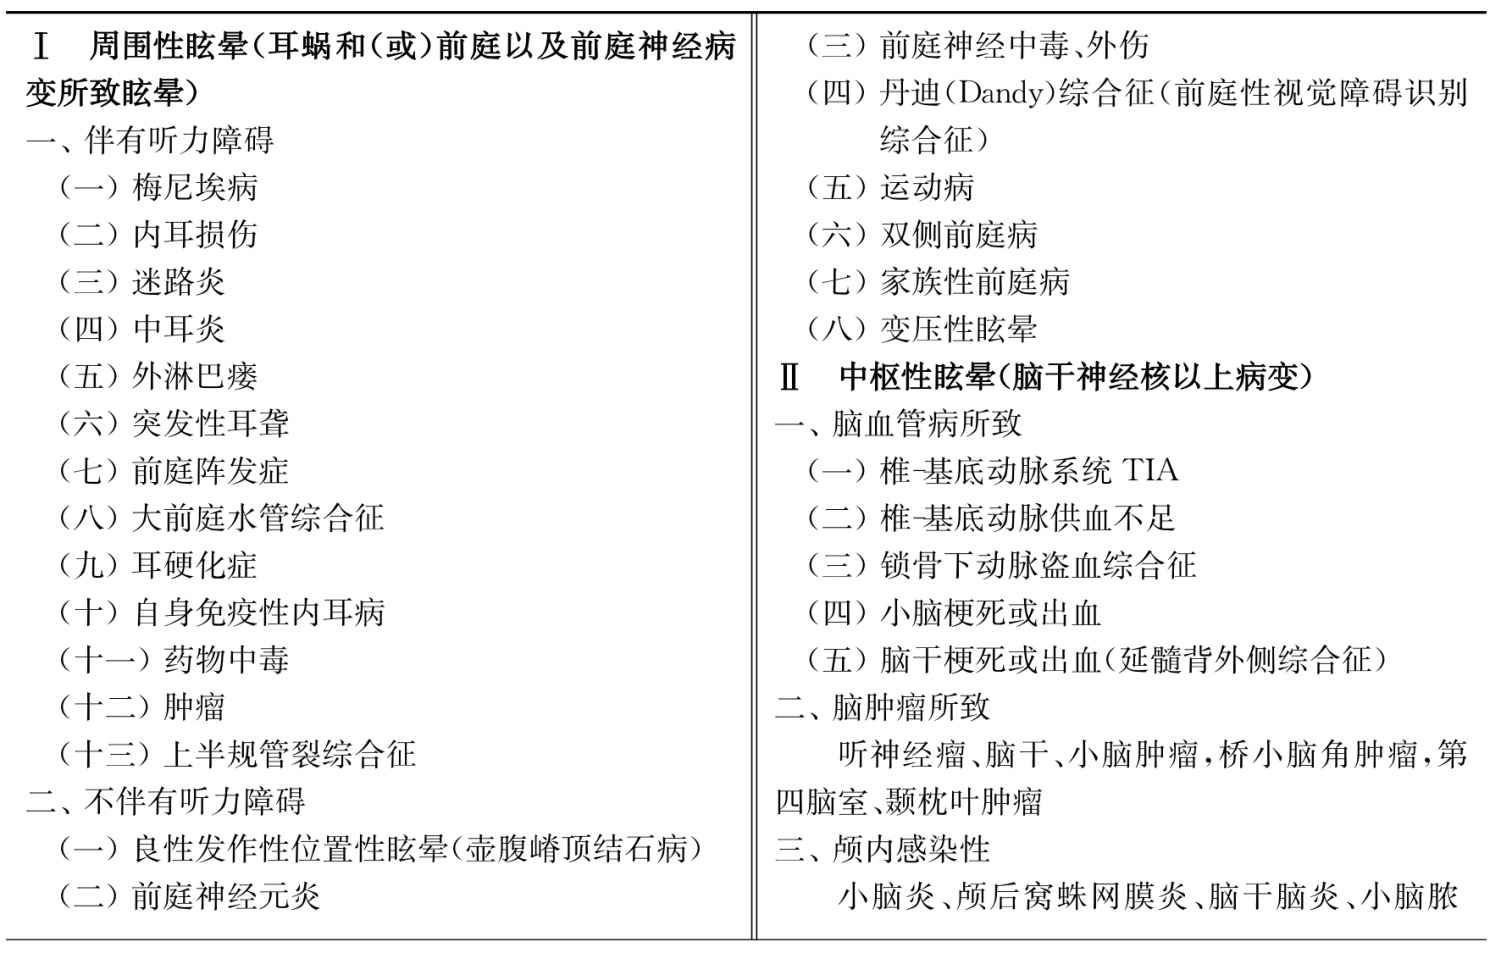
\includegraphics[width=\textwidth,height=\textheight,keepaspectratio]{./images/Image00295.jpg}\\
 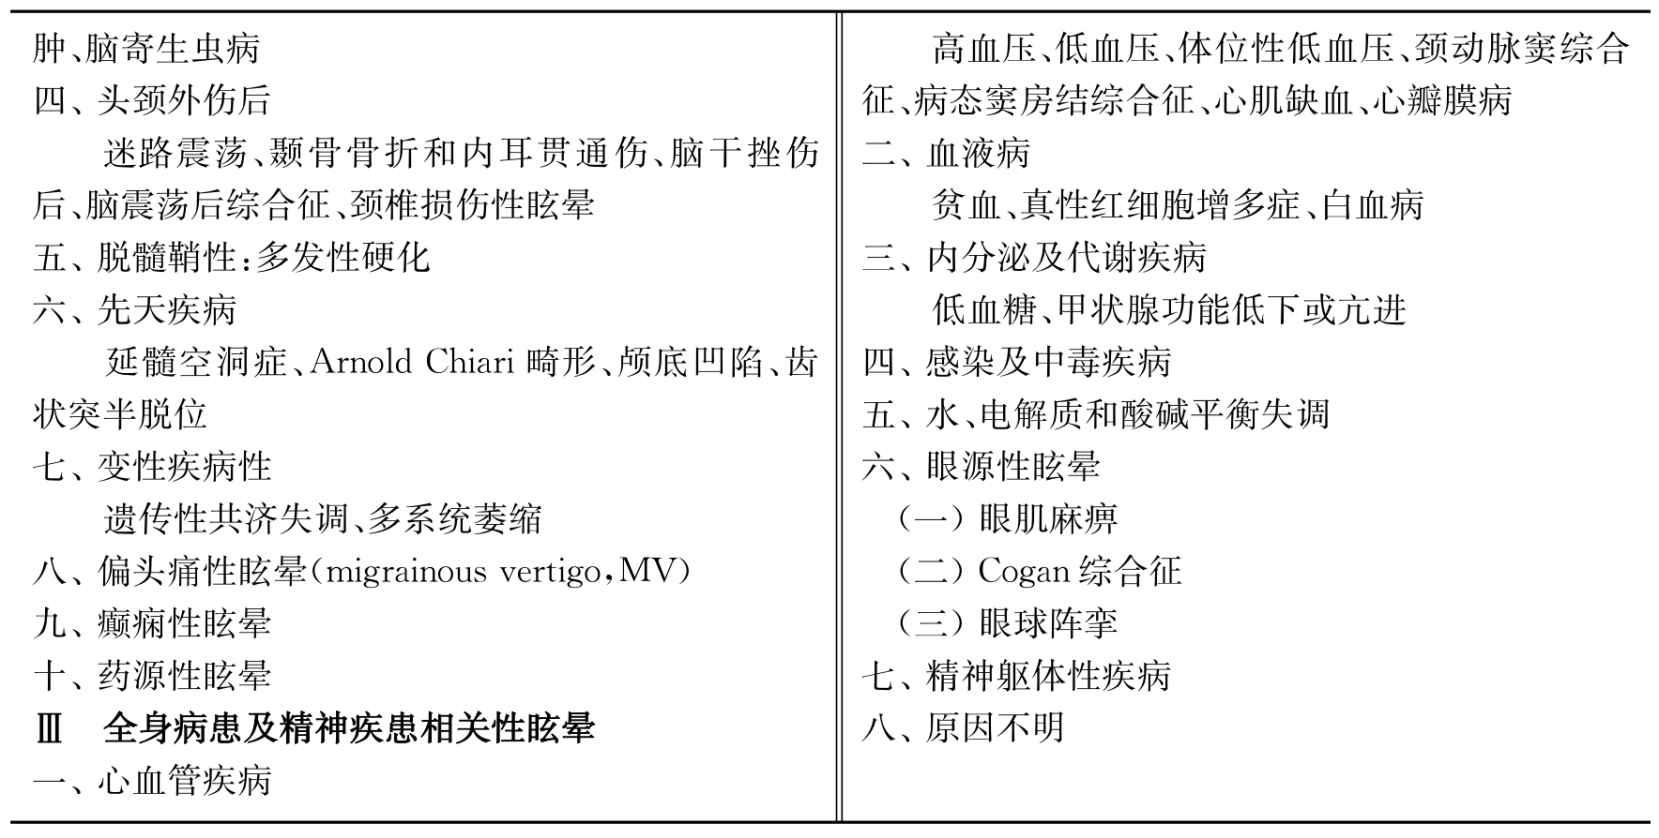
\includegraphics[width=\textwidth,height=\textheight,keepaspectratio]{./images/Image00296.jpg}
 \end{longtable}

\section{【眩晕的表现】}

眩晕最重要的特征是必须有运动的感觉,典型的运动感觉是旋转感,其他有晃动感、摇摆感、上升或下沉感、地动感、侧拉感、地面倾斜感、坐小艇感等。眩晕发作时大多数患者只能卧床,头部不动及闭眼可使症状减轻;反之可加重眩晕。常伴以眼球震颤(前庭神经核通过内侧纵束与眼肌联系);姿势不稳或倾倒以及偏过定位(前庭神经核通过前庭脊髓束、小脑红核脊髓束与脊髓前角细胞联系);迷走神经激惹症状如恶心、呕吐、面色苍白、出冷汗和血压改变(前庭神经核与脑干内迷走神经核和血管运动中枢联系)。下列分述各类型眩晕的特点。

\subsection{(一)耳性眩晕}

耳性眩晕是由迷路病变所致。这是一种典型的眩晕,具有明显的外周景物按一定方向旋转或自身的旋转感,持续时间较短,通常在数秒、数分钟至十多分钟停止,但可在数天内多次发作。眩晕发作时往往伴以:①水平性眼球震颤(其性质属于外周性眼球震颤,见表\ref{tab47-2});②姿势不稳或倾倒以及偏过定位;③迷走神经激惹症状较明显。如耳蜗器同时受累则伴有耳鸣和听力减退,本型眩晕的典型表现见于梅尼埃病;只有眩晕而耳蜗器不受影响者多见于壶腹嵴顶结石病。

\begin{table}[htbp]
\centering
\caption{外周型眼震与中枢型眼震的鉴别}
\label{tab47-2}
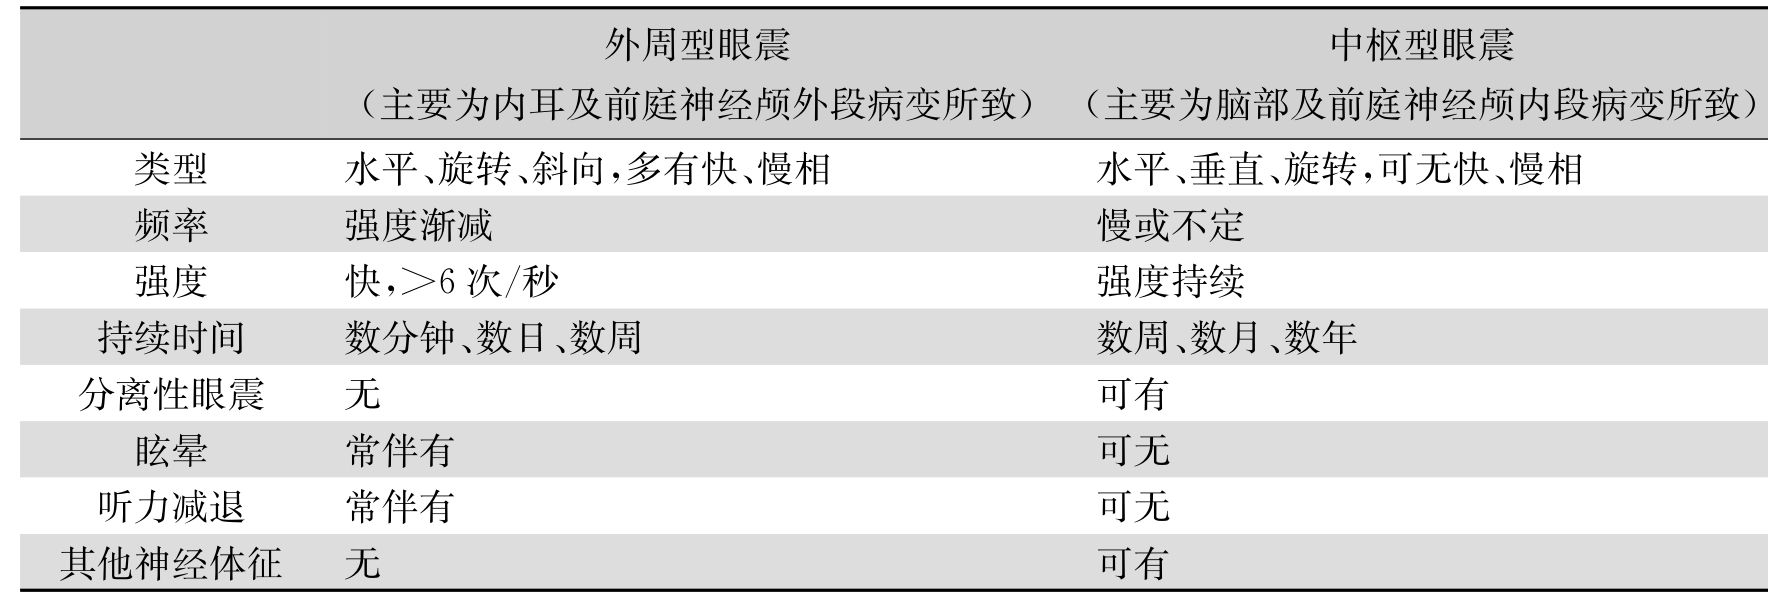
\includegraphics[width=5.94792in,height=2.03125in]{./images/Image00297.jpg}
\end{table}

\subsection{(二)前庭神经性眩晕}

前庭神经性眩晕可分为前庭神经颅外段(耳段)和前庭神经颅内段病变所致,前者的眩晕性质与耳性眩晕相似(一般较轻),但持续时间较长,如前庭神经元炎(眩晕持续数周)、药物中毒性内耳疾病(眩晕持续数月),发病开始时可伴有外周性眼震、姿势不稳以及迷走神经激惹症状,随病程渐长这些症状也逐渐消减。药物中毒性神经病如同时损害耳蜗神经也可发生听力减退甚至全聋,早期还可有耳鸣。前庭神经颅内段病变的眩晕主要指脑底的前庭神经病变引起者,常见的是小脑脑桥角肿瘤和蛛网膜炎,前者尤其是听神经瘤,早期常有病侧耳鸣及听力减弱,眩晕的发生多为慢性或亚急性,轻至中度,病程进展中逐渐出现同侧第5、6、7脑神经损害、同侧小脑征以及对侧锥体束征(脑干损害),并出现眼球震颤。小脑脑桥角蛛网膜炎较少见,其病征与小脑脑桥角肿瘤相似,但病程中缓解和复发比肿瘤明显。

\subsection{(三)前庭神经核性眩晕}

前庭神经核性眩晕是由于脑干的前庭神经核病变所致,眩晕可急起且剧烈(如延髓背外侧综合征);也可慢性发生、逐渐加剧(如脑干肿瘤)。常伴有眼震,其方向可为水平性、旋转性或垂直性,并可伴有邻近脑神经核以及上行性或下行性长传导束受累的病征,但不伴耳蜗症状,也很少伴发迷走神经激惹征。

\subsection{(四)脑干性眩晕}

脑干性眩晕是由于脑干病变损害了脑干内前庭神经核及其传入和传出纤维束,眩晕一般较轻,可伴有眼球震颤(水平性、旋转性、垂直性),如出现垂直性眼震则病变部位几乎可确定在脑干下部。不伴听觉障碍,可因病变不同而出现邻近神经核和长传导束受累的病征。这种眩晕可见于脑干肿瘤、脑干脑炎、脱髓鞘病、先天性和变性病。

\subsection{(五)小脑性眩晕}

小脑性眩晕是由于病变损害了小脑的绒球小结叶及其传入和传出纤维束,可引起急性眩晕(如出血或梗死)、亚急性眩晕(如亚急性小脑变性)、慢性持续性眩晕(如慢性药物中毒、肿瘤),眩晕的程度因其病变性质可为轻至重度,伴随较明显的姿位不稳、偏过定位、眼球震颤,很少伴有恶心、呕吐、耳鸣、听力减退等(但如小脑病变导致颅内压增高则可出现恶心、呕吐等)。小脑性眼震的特点为振幅较大,速度较慢,不规律,多为水平性,也可有混合性或斜向性,向病灶侧注视时眼震最明显。

\subsection{(六)大脑性眩晕}

大脑性眩晕是由于前庭皮质区(颞上回)病变所引起,眩晕的特点是强度较轻,有时呈发作性(癫痫先兆或癫痫发作),不伴恶心、呕吐、出汗、姿位不稳,眼震也少见,但可伴有邻近大脑结构性受累的表现。

\subsection{(七)颈性眩晕}

常发生于颈部突然转动时,患者出现明显的眩晕,颈部恢复中立位后眩晕消失。原因可能有:①颈椎骨质、颈椎关节、横突孔增生及骨赘形成;颈肌、颈部软组织病变;颈部肿物等或颅底畸形引起椎动脉受压而发生缺血,导致眩晕。如椎动脉本身有病变(粥样硬化性狭窄、畸形等),则症状更易发生。这部分发生症状的原因与椎基底动脉供血不足相似;②颈交感神经丛受直接或间接刺激,引起椎动脉痉挛或反射性引起内耳微循环障碍而发病;③颈反射异常,寰枕关节及上三个颈椎关节囊中的颈反射感受器受到各种刺激,其冲动可经颈1~3神经后根、脊髓小脑束、网状小脑束、橄榄小脑束等传至小脑或前庭神经核,产生眩晕及平衡障碍。

本症目前尚没有统一标准,一般采取排除法诊断。至少应有以下特征:①头晕或眩晕伴随颈部疼痛;②头晕或眩晕多出现在颈部活动后;③部分患者颈扭转试验阳性;④颈部影像学检查异常,如颈椎反屈、椎体不稳、椎间盘突出等;⑤多有颈部外伤史;⑥排除了其他原因。

其他疾病如心血管病、贫血、眼肌麻痹等所致者在大多数情况下都表现为头晕,少数情况下表现为眩晕。

\section{【眩晕病因鉴别诊断的相关检查】}

\subsection{(一)前庭功能检查}

前庭功能障碍时可发生自发性的前庭症状,如眩晕、眼球震颤、平衡障碍、迷走神经激惹症状;也可通过多种试验诱发出这些症状,根据诱发试验时患者的反应特点可以判断其前庭功能状态(正常、亢进、迟钝、消失)。

\subsubsection{1.自发性眼球震颤的检查}

眼球震颤是眼球不自主、短促的往返摆动。前庭器受刺激所产生的眼震为慢相(眼球向某一方向缓慢移动)和快相(继慢相之后眼球迅速返回原位的跳动,是大脑皮质的代偿作用),临床以快相定为眼球震颤的方向。

检查时患者头部不动,双眼注视前方50cm处的目标,并向左侧、右侧、上、下、左上、左下、右上、右下注视,侧视的角度不应超过45°,否则可能诱发出生理性终位眼球震颤。继而交替遮盖一眼检查,遮盖一眼出现的眼球震颤称为单眼眼球震颤或潜伏性眼球震颤,往往是先天性或中枢性疾病所致。检查时应注意眼震有无快相与慢相之分,眼震的形式(水平性、垂直性、旋转性、斜动性、混合性),眼震的振幅、频率、强度和持续时间。根据这些特点以确定眼震的类型,从而协助判断其病因。几种类型的眼球震颤其特点如下:

\paragraph{(1)外周型眼震(前庭外周型眼震):}

主要见于内耳疾病。眼震多呈水平性或水平略带旋转性,有快、慢相之分,病变较轻时(刺激性)快相多向病灶侧;病变较重时(破坏性)快相多向健侧。眼震持续时间较短,为时数分钟、数日至数周。多伴有眩晕,其程度与眼震程度较一致,躯体多向眼震慢相侧倾倒,常伴有听力减退。引起外周型眼球震颤的疾病主要为耳石病变和前庭神经颅外段病变,前者又称为耳石源性眼球震颤。出现眼震时应注意其方向、程度、持续时间等。耳石功能正常时,任何头位均不出现眼震;球囊体或球囊角耳石功能增高或不对称时,可出现水平性眼震。耳石源性眼震的特点是:眼震持续至头位纠正时为止,有较短的潜伏期,有一定的方向性,病程久则因中枢代偿而消失。

\paragraph{(2)中枢型眼震(前庭中枢型眼震):}

主要见于脑干、小脑、内侧纵束的疾病。眼震可呈水平、旋转、垂直或混合性(如为垂直性眼震则提示病变在脑干下部),眼震方向不定,有时并无快、慢相之分,可持续数月至数年。眼震不一定伴有眩晕,两者的程度不一致,眼震方向与躯体倾倒方向无一定关系,多不伴有听力减退。在中枢型眼震中还有两种比较特殊的眼震:①小脑性眼震,其特点已如上述;②内侧纵束性眼震,如内侧纵束有病变,可破坏双眼的协调性共同运动,出现分离性眼震(一眼向内下、一眼向外上),两侧眼震的程度不等。外周型眼震与中枢型眼震的鉴别见表\ref{tab47-3}。

\subsubsection{2.前庭诱发试验}

是用各种方法刺激半规管,借以诱发眩晕、眼球震颤、倾倒、偏过定位、自主神经症状,以判断前庭功能状态。常用的方法有冷热试验(也称变温试验)、旋转试验、位置试验、视动性眼震试验、眼震电图检查(包括扫视试验、平稳跟踪试验和视动性眼震试验、凝视试验、静态位置试验、动态位置试验和冷热试验)、平衡试验(Romberg征、Mann试验、直线试验)等。

\begin{table}[htbp]
\centering
\caption{外周型(良性)与中枢型(恶性)位置性眼震的鉴别}
\label{tab47-3}
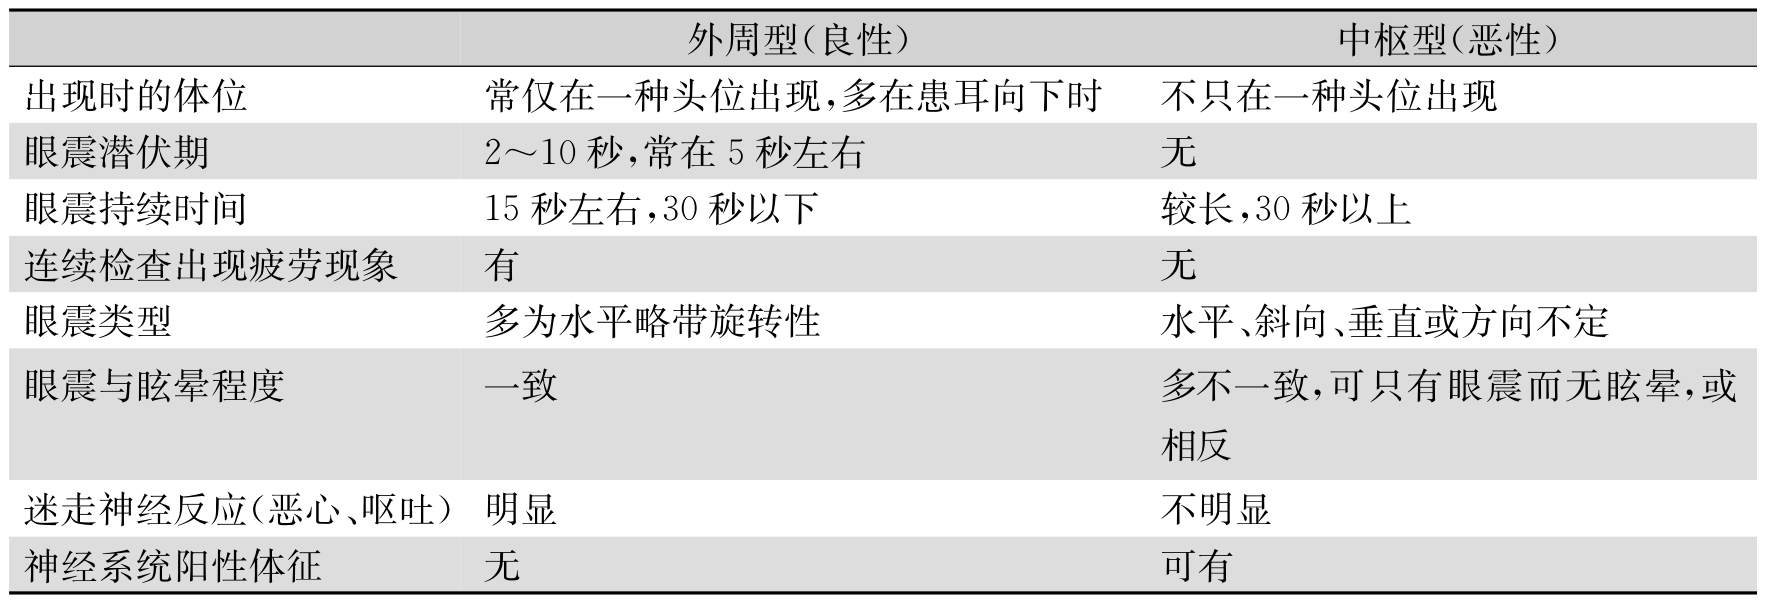
\includegraphics[width=5.88542in,height=2.02083in]{./images/Image00298.jpg}
\end{table}

\subsubsection{3.位置性眼震和眩晕}

当头部处于某一种或某几种特定位置时出现的眼球震颤及眩晕,称为位置性眼震和眩晕。位置性眼震及眩晕有两型:①外周型,也称良性位置性眼震及眩晕,大多由于内耳的前庭疾病所引起;②中枢型,也称恶性位置性眼震及眩晕,常由于颅后窝病变尤其是颅后窝肿瘤、多发性硬化、椎-基底动脉供血不足、颅脑损伤等引起。两型各有其特点,可通过位置性试验(Dix-Hallpike或Roll
test)给予初步鉴别(表\ref{tab47-3})。检查方法:患者坐于检查台上,检查者以双手固定患者头部,患者双目注视检查者前额。然后让患者仰卧,观察其有无眼球震颤,如10~15秒仍无反应,则让患者坐起再观察10~15秒。随后以同样的步骤让患者左侧卧、右侧卧、仰卧头低30°等观察有否眼震。患者头位变动至出现眼震的时间称为位置性眼震的潜伏期,一般为5~20秒。诱发的眩晕和眼震一般持续在1分钟之内,表现为“由弱渐强------再逐渐弱”;患者由卧位坐起时,常出现“反向眼震”。

\subsection{(二)听力检查}

\subsubsection{1.阈上听力检查}

是鉴别耳蜗性聋与蜗后性聋的方法之一,同时做重振试验。

\subsubsection{2.声阻抗测定法}

不仅可测试中耳的传音功能,而且通过错骨肌反射的测试,可以了解脑干听觉通路的状况。

\subsubsection{3.脑干听觉诱发电位(BAEP)}

对蜗后、脑干病变的诊断较有帮助。

\subsection{(三)电生理检查}

包括脑电图、视频脑电图、听觉诱发电位(BAEP)、视觉诱发电位(VEP)、眼震电图、耳蜗电图。

\subsection{(四)神经影像学}

包括X线平片、CT、MRI、FMRI、MRA、CTA等。

\subsection{(五)其他}

SPECT、PET、CT+PET、TCD、DSA、脑脊液、脑磁图等。

\section{【眩晕鉴别诊断的思路】}

\subsection{(一)首先确定是否眩晕}

通常依据典型的、有运动感的眩晕发作,常表现以突发性和间歇性的外物和(或)自身旋转、翻滚、浮沉或飘移感(闭眼不缓解)为主要症状,伴眼球震颤及迷走神经激惹症状,临床上可诊断为眩晕。

在诊断过程中需与头晕(dizziness)鉴别,头晕多表现为头轻目眩感、眼花、头脑麻木或空虚感、脚步轻浮感或摇晃不稳感,而无运动的感觉;一般不伴眼球震颤、倾倒、偏过定位,无或仅有轻微迷走神经激惹症状;前庭功能检查正常。

眼部疾患和系统性疾病(如心脏病、贫血等)以及深感觉障碍疾病常引起头晕,而较少引起眩晕。

头晕也可见于小脑性共济失调引起的失平衡和摇摆的感觉,是由于小脑组织中除了绒球、小结叶以外的部位损害所引起。

耳石功能障碍也可引起头晕,其特点是多在头部作直线运动时出现,如蹲下、起立、行走等(椭圆囊耳石有病变);头晕也可出现于左右摆头或卧位侧翻身(球囊体耳石有病变)。

此外,头晕常见于一些精神、心理及外伤性疾病,如抑郁症、焦虑症、更年期综合征以及脑震荡后遗症等患者,其症状较长时间存在或反复出现,可伴恶心或自主神经紊乱症状。往往伴有大脑皮质功能减弱的其他表现,如头痛、失眠、多梦、记忆力减退、注意力不集中、倦乏等。头晕的程度常与情绪不稳、紧张或疲劳相平行。体检常无异常发现。

另外,还需与晕厥(syncope)鉴别,尤其是晕厥发作前的感觉意识要丧失和黑蒙也会使患者感觉头晕或眩晕。

\subsection{(二)判断导致眩晕的病变部位及病因}

\subsubsection{1.详细了解病史及眩晕的特点}

发作的形式和频率:急性或慢性,频率是单次、首次或复发性;发作的持续时间;数秒、数分钟、20分钟以上、数天或持续性;诱发因素及与体位的关系:是否由于头位或颈位与体位的改变而诱发?是否与月经、睡眠剥夺、瓦氏动作、视野中物体的运动有关?发作时能否站稳或向何方倾跌;伴随症状:有否听力下降、耳鸣、耳胀?是否伴有自主神经症状?是否有复视、构音障碍、共济失调等中枢神经症状?是否有微光、头痛、视觉先兆等。

\subsubsection{2.详细了解过去史}

既往用药史,特别是有否使用容易引起内耳中毒的药物如链霉素类、容易引起中枢损害的药物如镇静、安定、麻醉药和苯妥英钠等。其他病史如头颈部外伤史、耳部和眼部疾病史、心血管病、内分泌及代谢病史、血液病史。有否眩晕的家族史。

\subsubsection{3.体格检查和相关的辅助检查}

\paragraph{(1)体格检查:}

最重要的是神经系统和耳部,应重视前庭功能检查。内科尤其是心血管、血液系统检查不能忽视。

\paragraph{(2)实验室检查:}

项目繁多,可选择需要者行之。在神经影像学的多项检查中,MRI是中枢性眩晕的首选检查。业已证明颅后窝病变(如小脑脑桥角病变)最敏感的方法是对比增强MRI。对疑为多发性硬化的炎性脱髓鞘病灶所致的眩晕,首选的检查必定是MRI。此外,MRA是发现基底动脉和椎动脉梗死的好方法,但有时会出现假象,其分辨率不如血管造影(DSA),故必要时可进行选择性后循环的血管造影以助诊断。检查迷路的病变采用MRI有其优点,因MRI的分辨率高,还可用特殊序列增强以观察迷路内液体的情况,帮助医生能更细致地分析迷路病变。对梅尼埃病进行MRI检查可发现的特征性改变是病变侧内淋巴管和内淋巴囊萎缩,后半规管和后窝之间的骨密度降低。怀疑中耳炎引起的眩晕或外伤后眩晕都要求使用高分辨率CT检查,以了解骨骼的情况。

\subsubsection{4.综合分析病变部位和病因}

综合病史、阳性体征、辅助检查的结果,进一步考虑眩晕属于前庭系统性或非前庭系统性,如属前者,应尽可能鉴别是迷路或前庭神经颅外段的病变所引起,抑或前庭神经颅内段、前庭神经核、小脑、脑干、大脑前庭中枢以及它们的上、下行联系束病变所引起。进而确定病因。临床上常需着重下列两个方面的鉴别:

\paragraph{(1)前庭系统的外周性(耳性)与前庭系统的中枢性(脑性)眩晕的鉴别:}

见表\ref{tab47-4}。

\begin{longtable}{c}
 \caption{前庭系统的外周性与前庭系统的中枢性眩晕的鉴别}
 \label{tab47-4}
 \endfirsthead
 \caption[]{前庭系统的外周性与前庭系统的中枢性眩晕的鉴别}
 \endhead
 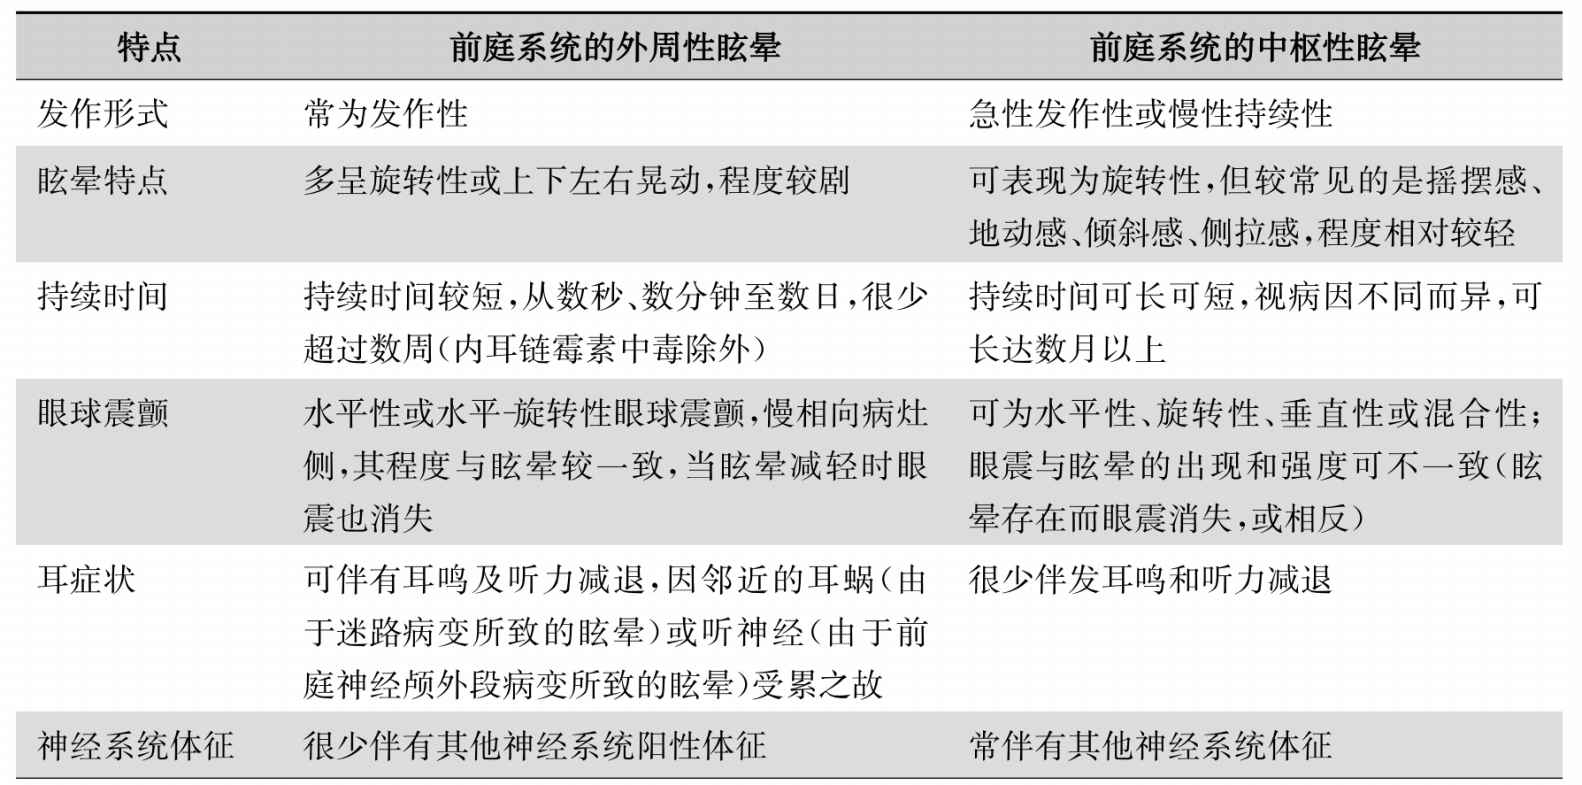
\includegraphics[width=\textwidth,height=\textheight,keepaspectratio]{./images/Image00299.jpg}\\
 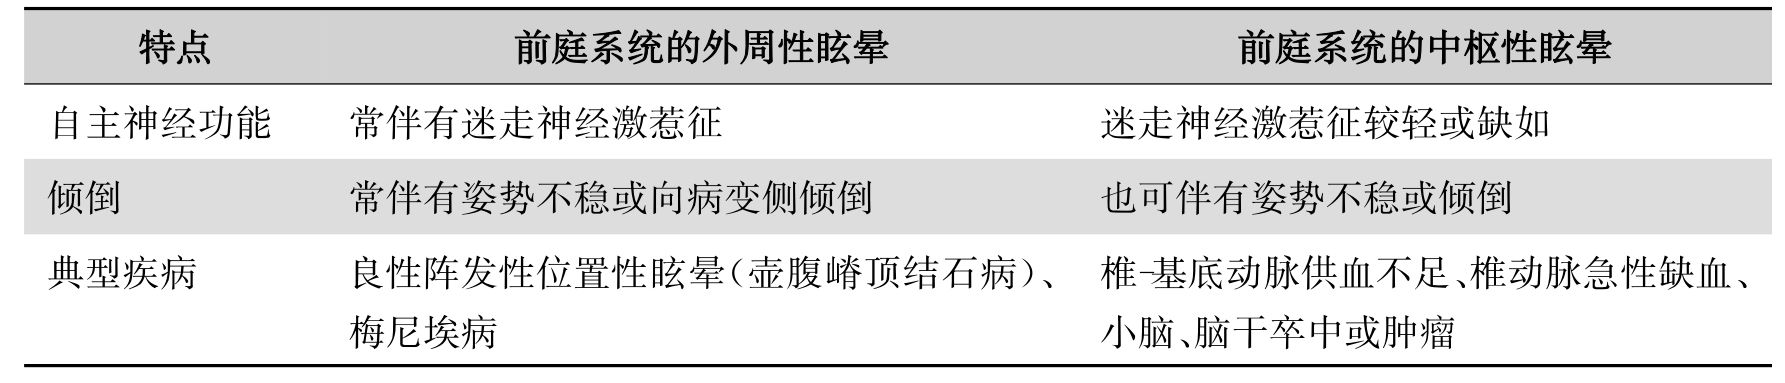
\includegraphics[width=\textwidth,height=\textheight,keepaspectratio]{./images/Image00300.jpg}
 \end{longtable}

临床上常遇到一类发作性眩晕,表现为突然发生,在仰卧位或侧卧位突然起坐或急剧转头时最易出现,眩晕有旋转感或其他运动感,可伴恶心、呕吐,但罕有伴发耳鸣,持续时间多为几秒、几十秒,很少超过几分钟。在数天、数周甚至数月内反复发作。临床上对这类眩晕的诊断往往含糊甚至混乱,较多诊断为椎-基底动脉供血不足,或者是颈性眩晕、良性位置性眩晕(壶腹嵴顶结石病),也有诊断为梅尼埃病。事实上这种表现的眩晕均可见于前三种疾病,但以良性位置性眩晕多见(其特征见后述)。

\paragraph{(2)对眩晕病因诊断的一些线索:}

1)眩晕发生的年龄:①儿童:常发生眩晕,急性者见于急性小脑炎;如反复发作性,考虑有否儿童期良性发作性眩晕(或偏头痛性眩晕,参见第46章)。慢性进展性,需考虑颅后窝占位性病变或蛛网膜囊肿、苯妥英钠中毒;②青年:颅内各种疾病,头颈外伤,苯妥英钠中毒;③中年:梅尼埃病(10~50岁);前庭神经元炎(30~60岁);良性发作性位置性眩晕(中年后);④老年:良性发作性位置性眩晕,Dandy综合征,脑血管病性眩晕(常见的是椎-基底动脉供血不足、颈性眩晕)。老年人由于迷路感觉、本体感觉以及视觉的结构退化导致传入冲动减少或不对称,同时中枢控制功能也减弱,因而易发生眩晕和平衡障碍。

2)眩晕的起病形式及病程经过:①急性,复发性,极短暂性,反复发作数周至数月:良性发作性位置性眩晕(壶腹嵴顶结石病);②急性,复发性(有或无),短暂性,持续两周左右:梅尼埃病;③急性,单次发作(可有复发):脑血管病性眩晕;④急性发生、慢性经过:头颈部外伤性眩晕;⑤急性或亚急性发生,好转或恶化:脑部感染,脑脓肿;⑥慢性,进展性:颅内占位病变(主要是小脑脑桥角肿瘤、脑干肿瘤、小脑肿瘤、第四脑室肿瘤等);⑦慢性发生,慢性过程,可缓解或加重:慢性颅内高压症;⑧慢性进展性,可有缓解及复发:多发性硬化(由于第四脑室前庭神经进入颅内处的斑块所引起);⑨慢性发生,较缓慢发展:橄榄脑桥小脑萎缩(OPCA),脊髓小脑性共济失调(SCA);⑩亚急性进展至高峰,可缓解:亚急性小脑病(副肿瘤综合征)。

3)伴随症状:①伴有耳蜗症状:梅尼埃病,内耳药物中毒,小脑脑桥角肿瘤、内听动脉病变;②伴有轻微或不伴有耳蜗症状:椎-基底动脉供血不足,颈性眩晕;③不伴有耳蜗症状:良性发作性位置性眩晕,前庭神经元炎,Wallenberg综合征,脑干或颅后窝肿瘤;④伴有恶心、呕吐:梅尼埃病、前庭神经元炎、前庭动脉病变、颅内占位性病变、颅内高压症;⑤除了第8脑神经之外还出现其他神经症状:小脑脑桥角肿瘤,脑内其他结构性病变所致的眩晕;⑥伴有较明显的头痛:颅内占位性、血管性、感染性、外伤性疾病,颅内高压症;⑦伴明显眼花及黑蒙:Dandy综合征。

几种以眩晕为主要症状的疾病的鉴别见表\ref{tab47-5}。

\begin{table}[htbp]
\centering
\caption{几种眩晕疾病的鉴别}
\label{tab47-5}
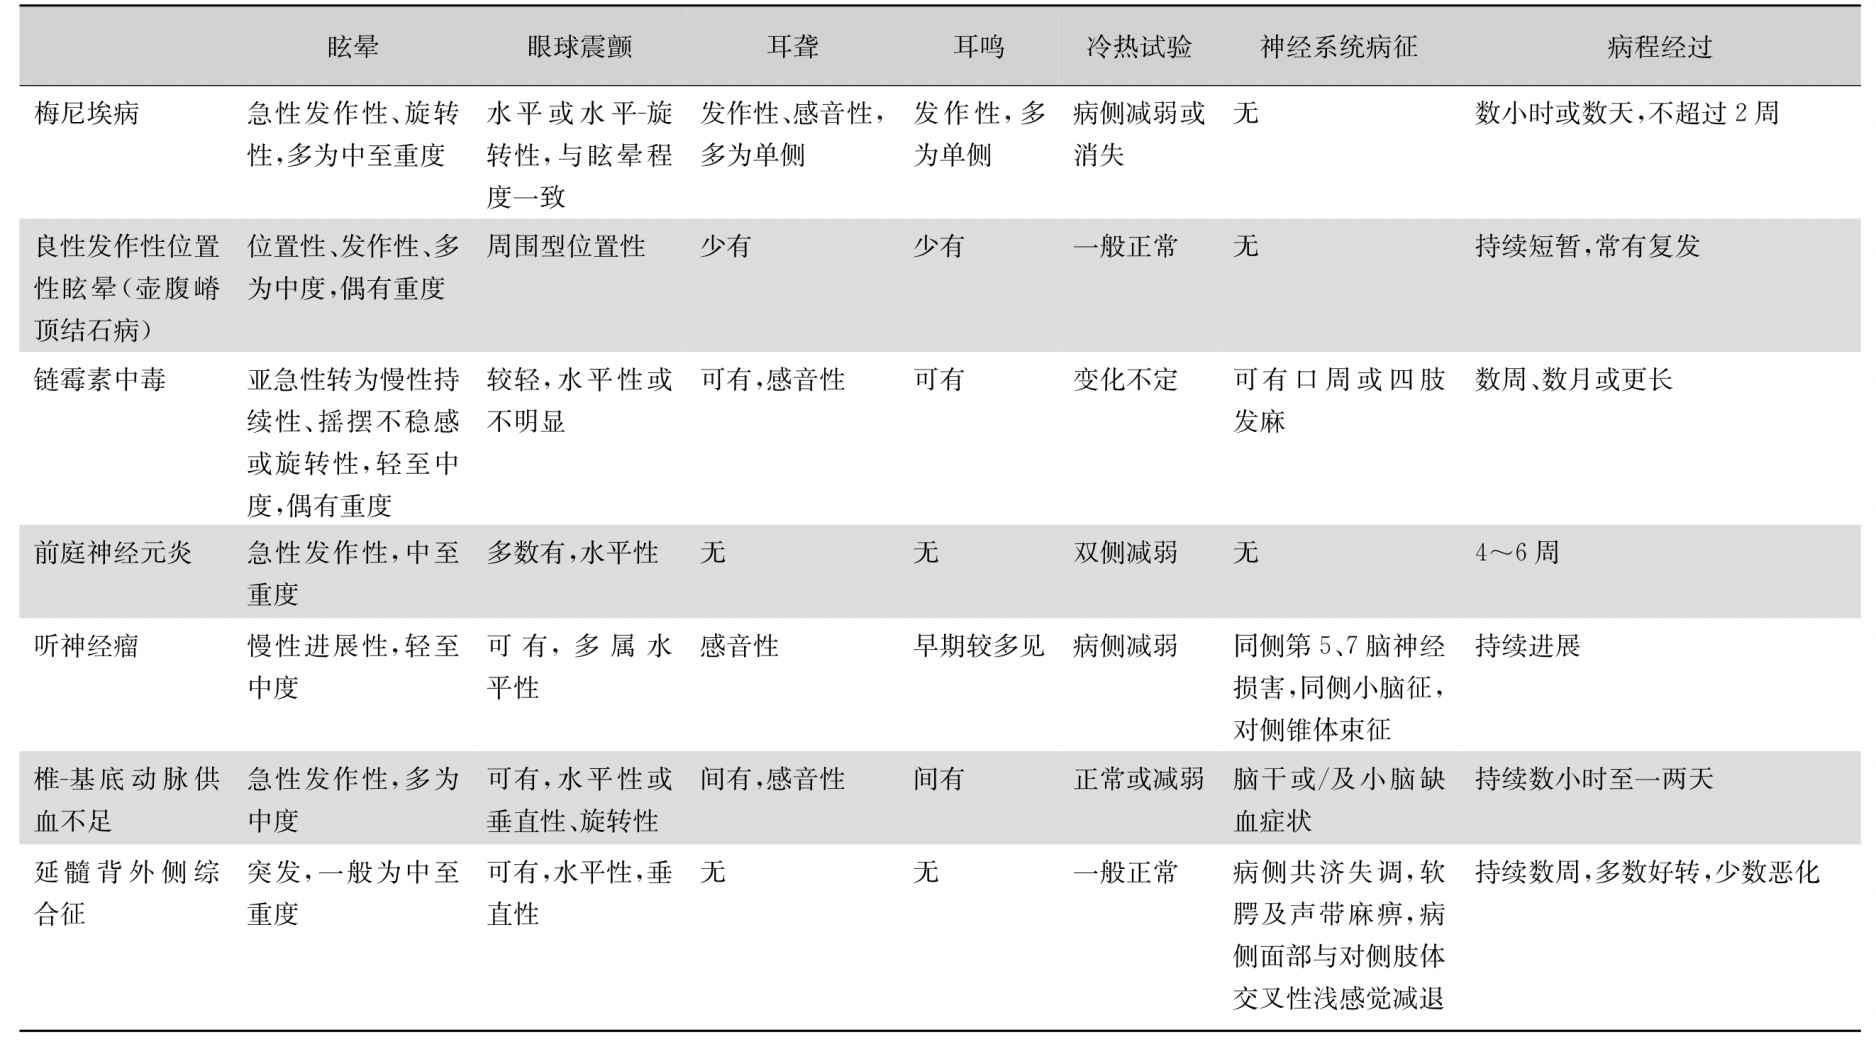
\includegraphics[width=8.8125in,height=4.91667in]{./images/Image00301.jpg}
\end{table}

\protect\hypertarget{text00359.html}{}{}

\section{157 周围型眩晕}

由于脑干神经核以下[耳蜗和(或)前庭以及前庭神经)]病变所致眩晕,绝大多数系耳部疾患引起,除眼震和有时可能伴听力障碍之外,患者没有相关的神经系统损害的症状和体征。

\subsection{157.1 伴有听力障碍的周围性眩晕}

\subsubsection{一、梅尼埃病(Méniére disease)}

本病又名膜迷路积水、内耳眩晕病。发病机制是由于内淋巴分泌过多或吸收障碍,引起膜迷路积水,淋巴压力因而增高,导致内淋巴腔扩大以及内耳末梢器缺氧变性所致。关于产生膜迷路积水的原因则有多种学说,较多人支持神经-血管障碍学说,即认为自主神经调节障碍引起内听动脉痉挛、微循环障碍,影响内淋巴的分泌吸收。其他学说包括:内耳变态反应学说,使血管壁渗透性增高而致局部水肿;发作性椭圆囊和半规管膜破裂伴淋巴液外渗学说,使高钾的内淋巴液和高钠的外淋巴液混合,刺激和破坏内耳的感觉细胞和神经;内分泌障碍学说,主要是肾上腺皮质功能不全或甲状腺功能减退,引起内耳的组织代谢降低,导致内淋巴吸收障碍;代谢障碍学说,认为酶活动异常,以致内淋巴的蛋白水解过程不完全;感染学说,尤其是上呼吸道感染;维生素缺乏学说;电解质和水的平衡障碍学说,因本病发作时血清钾离子增高,镁离子下降。所有这些学说均未得到充分证实。

\paragraph{(一)临床特点}

本病好发于中年人,儿童及老人间有发生,男女罹病大致相等,或呈3∶2。多为单耳受累,约10\%的病例累及双耳。发作通常无明显诱因,也可由于疲劳、焦虑而诱发。不少患者在发作前数周、数日或数小时出现患耳胀满感、重压感、耳后钝痛等前驱症状,典型临床表现是发作性眩晕、波动性耳聋、耳鸣三联症。眩晕可在任何时间突然发作,常呈旋转性,程度颇剧,伴有身体不稳或向一侧倾跌,因而患者不能走路或站立,闭目静卧于某一位置可使眩晕减轻,睁眼或头部略移动使眩晕加重。眩晕多持续数分钟至数小时渐消退,但仍在数日内遗留轻微头晕不稳感。眩晕常伴恶心、呕吐、出汗、面色苍白和血压下降。耳鸣及耳聋与眩晕同时出现者大约见于50\%的病例,另有约25\%的病例在眩晕出现前、25\%的病例在眩晕出现后才发生耳鸣及耳聋。耳鸣初时多数为低音调,以后可转为持续高音调,眩晕消失后耳鸣也渐消失,听力则有部分恢复。发作时意识清晰,罕见病例有短暂的意识丧失而误诊为癫痫。眩晕发作时可出现水平略带旋转的眼球震颤,向患侧注视明显,眼震与眩晕的出现及程度比较一致,随眩晕缓解眼震也消失。本病发作频度不等,重者每周发作数次,也有终生仅发作一次,间歇期通常为数月至数年。多次发作后眩晕程度渐减而耳聋渐重,待完全耳聋后眩晕发作可终止。

\paragraph{(二)辅助检查}

\subparagraph{1.甘油试验}

于发病时检查,方法是以95\%的甘油(0.5~1.5ml/kg体重)加生理盐水一倍顿服,分别在服前、服后1、2、3小时检查听力变化,约70\%的患者听力改善约15dB。

\subparagraph{2.变温试验(冷热水试验)}

可见患侧前庭功能减退。

\subparagraph{3.重振实验}

大约60\%的患者呈阳性。

\subparagraph{4.耳蜗电图}

Sp/Ap>0.40,提示淋巴内水肿。

\subparagraph{5.MRI检查}

可发现的特征性改变是病变侧内淋巴管和内淋巴囊萎缩,后半规管和颅后窝之间的骨密度降低。

\paragraph{(三)诊断和鉴别诊断}

\subparagraph{1.诊断要点}

中年人多见,突然发生内耳三联症:发作性眩晕、波动性耳聋、耳鸣,很多患者有患耳胀满或重压感,上述各种辅助检查可帮助诊断。

\subparagraph{2.鉴别诊断}

梅尼埃病应与迷路炎、良性位置性眩晕、前庭神经元炎、内耳药物中毒、椎-基底动脉供血不足等病鉴别(见表\ref{tab47-5})。另外,临床上有一种少见的发作性眩晕病,称为雷梦耶综合征(Lermoyez
syndrome),也会与梅尼埃病混淆,不过前者发病时先出现病侧耳鸣、耳聋,继后出现眩晕,眩晕发生后耳鸣和耳聋逐渐恢复,眩晕持续10~20分钟后也逐渐消失。所以Lermoyez综合征也称为耳鸣-耳聋-眩晕综合征。其发生机制可能是病变先堵塞了蜗管和球囊间的连合管,蜗管内的内淋巴压力升高,影响听觉神经末梢;继后半规管内淋巴压力上升刺激壶腹嵴顶的前庭神经末梢才出现眩晕发作。梅尼埃病与Lermoyez综合征的鉴别是眩晕出现在前,然后才出现耳鸣和耳聋,眩晕持续时间也较长。

\subsubsection{二、迷路炎(labyrinthitis)}

迷路炎是由于耳部感染累及骨迷路及膜迷路所致的眩晕,四种迷路炎(弥漫性浆液性迷路炎、弥漫性化脓性迷路炎、病毒性迷路炎、药物中毒性迷路炎)都可引起眩晕,但以前两者引起的眩晕最重。临床上对于急性或反复出现的外周性眩晕,应注意有否迷路炎症。

\subsubsection{三、外淋巴瘘}

外淋巴瘘是指膜迷路周围的外淋巴与中耳腔之间的异常通道,使外淋巴逸出内耳而引起听力障碍和(或)平衡障碍。据统计,外淋巴瘘人群发病率为1/10万,约占突聋患者的10\%,目前临床对本病的认识不十分清楚,小儿与成年人发病病因有差异,小儿双侧发病率较成年人高,在大多数病例中其发生与中耳或内耳畸形有关。

\paragraph{(一)病因和发病机制}

可按先天性和后天性分类如下:

\subparagraph{1.先天性}

内耳骨性包囊的孤立缺损:镫骨底板瘘,圆窗畸形,内听道的筛状板缺损,窗前裂未闭,岩大神经管裂孔畸形等。先天性外淋巴瘘伴颞骨或颅外畸形:Mondini型内耳发育不全,蜗小管宽大而开放,前庭小管扩大,先天愚型等。

\subparagraph{2.后天性}

\hypertarget{text00359.htmlux5cux23CHP47-5-1-3-1-2-1}{}
(1)外伤性:

中耳和内耳直接穿通伤,闭合性头颅外伤或头颅钝挫伤,耳创伤,气压伤,中耳和乳突手术直接损伤或通过听骨链间接损伤镫骨。

\hypertarget{text00359.htmlux5cux23CHP47-5-1-3-1-2-2}{}
(2)肿瘤和感染:

内耳骨性包囊被中耳乳突胆脂瘤、肿瘤或梅毒侵犯。

\hypertarget{text00359.htmlux5cux23CHP47-5-1-3-1-2-3}{}
(3)特发性外淋巴瘘:

无外伤、气压创伤史,亦无耳部手术史,由于中耳或蛛网膜下腔(脑脊液)压力的急剧变化,如用力擤鼻、大便、剧咳,从事需用力屏气的体力劳动(如抬举重物等)引起。

本病引起感音神经性聋和眩晕的机制为:①双膜破裂后,使外淋巴向圆窗纵向流动导致广泛的内外淋巴混合,引起一系列生物化学和病理生理变化,使耳蜗感觉神经上皮功能严重受损;②外淋巴液流失,空气逸入外淋巴系,使内淋巴液流动受到干扰,对声波传导受到破坏,并对耳石器和壶腹终顶产生异常刺激;③继发性膜迷路水肿,螺旋器退变;④浆液性或纤维素性迷路炎。

\paragraph{(二)临床表现}

\subparagraph{1.听力障碍}

可发生于单耳或双耳,程度从轻度到重度,听力损失多为进行性或稳定的感音神经性聋,也可表现为波动性或突发性感音神经性聋。并发于手术者,多为术后出现波动性耳鸣,听力损失一般不重。如瘘管不能修复,耳聋则逐渐加重,言语接受阈升高,言语识别率下降。

\subparagraph{2.耳鸣、眩晕和平衡障碍}

发作性眩晕,平衡障碍或共济失调这些周围性前庭症状可单独出现或与感音神经性聋同时发生。特发性迷路窗膜破裂者,多有严重旋转性眩晕,伴恶心呕吐、冷汗等自主神经症状,卧床不起,日后眩晕逐渐减轻,但仍有平衡失调、不稳感。在瘘管修复前,此症状经久不愈。典型患者诉畏强声,听到强声时即有头晕、恶心感,系强音引起镫骨肌反射,使外淋巴液经卵圆窗漏出增多所致。外淋巴瘘大多数伴有耳鸣。

\paragraph{(三)诊断和鉴别诊断}

Kohut等指出,外淋巴瘘诊断应包括病理诊断资料,诊断方法包括三个方面:①查“洞”:通过影像检查、耳内镜及手术探查发现瘘管;②查“漏”:通过内镜、手术探查或通过外源性荧光素或内源性标记物(B2-转铁蛋白)查找外淋巴瘘的证据。近来有学者发现B2-转铁蛋白是脑脊液、玻璃体和外淋巴液才有的特殊蛋白质,主张用测定鼓室液体中的B2-转铁蛋白作为外淋巴瘘的诊断方法;③查外淋巴屡所致的反应变化:即ENG\textbackslash{}听力学检查及瘘管试验。

据临床经验,有如下情况者应疑为本病:①不明原因的突发性聋伴眩晕,经治疗后眩晕不减轻或虽有减轻,仍有平衡失调、位置性或变位性眩晕,如发病前有鼓室压或颅内压骤升者,更应高度疑为本病;②颅脑外伤后眩晕长期不愈,感音神经性聋逐渐加重者;③良性位置性眩晕,手术探查是确诊外淋巴瘘的重要手段,应作为外淋巴瘘诊断的常规方法。鼓室探查可确定迷路窗的“洞”或“漏”。

\subsubsection{四、突发性耳聋}

突发性感音神经性聋(简称突发性聋或突聋),是一种以短时间内听力明显下降为主要表现的综合征,部分病例伴有眩晕等不适。目前其具体病因、发病机制仍不明了。突聋的致病原因不清,与内耳微循环障碍、病毒感染、窗膜破裂、变态反应、血管纹功能不良及代谢障碍等有关,其中内耳血流障碍和病毒感染学说被普遍接受。无论是内耳血流障碍或病毒感染,最终都导致螺旋神经节、耳蜗内神经元及听毛细胞的供血障碍、营养缺乏,致神经萎缩、变性,引起感音功能减退甚至全聋。内耳供血系统的脆弱性及耳蜗与前庭供血部分同源性,当某种原因引起内耳血供障碍,极易导致内耳组织(包括耳蜗、前庭及半规管)水肿、缺血、缺氧、代谢紊乱,功能突然下降、甚至丧失而表现为突聋并伴或不伴眩晕。丁建慧等观察202例患者中有60例伴眩晕,142例不伴眩晕。

\subsubsection{五、前庭阵发症(vestibular paroxysmal,VP)}

是常见的眩晕疾病之一,约占眩晕疾病的4\%。病因可能与神经-血管交互压迫(NVCC)有关。血管压迫导致第8对脑神经局部脱髓鞘及继发的动作电位假突触传播,使受微血管波动性压迫的前庭神经活动信号异常放大,可能是其发病的主要病理机制。VP临床主要表现为反复的短暂的眩晕发作,持续数秒至数分钟,随着病程的延长,眩晕发作的频率增加,持续时间延长,可出现听觉过敏及耳鸣,少数患者仅表现为发作性耳鸣或听力下降而无眩晕症状。有报道前庭神经和血管交互压迫导致打字机式耳鸣。头颅MR增强扫描可了解颅内前庭神经和血管的关系,脑干听觉诱发电位检查也有助于诊断。

\subsubsection{六、大前庭水管综合征(large vestibular aqueduct syndrome,LVAS)}

又称先天性导水管扩大,是在20世纪70年代末随着CT的问世才被发现的一种新的致聋疾病,主要表现为幼儿波动性感音神经性耳聋和眩晕。1978年被正式命名为LVAS,是一种先天性遗传性疾病,一般认为是常染色体隐性遗传,除前庭导水管扩大外,不合并其他内耳畸形。

由于先天发育异常导致前庭导水管扩大时,内淋巴液可经扩大的前庭导水管从内淋巴囊倒流于耳蜗或前庭,损伤感觉毛细胞出现耳聋或眩晕。在耳部影像检查者中存在大前庭导水管者占1\%;患儿出生时听力一般接近正常,多数在3~4岁发病。感冒和外伤常常是发病的诱因,即使轻微的外伤也可引起重度感音神经性耳聋和眩晕;采用神经营养剂治疗,有一定效果,部分患儿的听力可恢复到原有水平,但仍较正常儿童听力差,听力容易波动,目前尚无特效的治疗方法。

早期发现采取防范措施,可延缓病情发展,患儿出生后听力接近正常,虽处于亚临床期,患儿说话较晚,口齿不清,上感或外伤后听力下降有时呈可逆性,及时行听力和平衡功能检查有助于诊断,做颞骨CT扫描检查可以确诊,早期证实此症并采取预防措施,特别是预防头部磕碰,有可能保持更多的听力储备。

\subsubsection{七、耳硬化症(otosclerosis)}

又名耳海绵化症(otospongiosis),是一种以原发性迷路包囊骨海绵样变性为病理特征的内耳疾病。其颞骨病理特征为骨迷路包囊灶性骨质吸收,髓腔扩大,血管增多,呈海绵样变,破骨、成骨现象可同时存在。临床耳硬化症的发病率随种族和地区不同而有所不同。白种人的发病率最高,为0.3\%~0.5\%,黄种人则被认为是此病的低发种族。然而,组织学上耳硬化症的发病率远比临床的发病率高,约为2.5\%。本病的男女发病率之比为1∶1.85,高发年龄为20~50岁,高峰在30~40岁之间。因病变侵犯的部位和范围不同,临床特征可表现为隐匿型、传导性聋、感音神经性聋及混合性聋,部分伴有眩晕症状。

病灶接近前庭窗、侵犯环韧带及镫骨板者,表现为传导性聋;病灶侵犯蜗管表现为感音神经性聋或混合性聋,侵犯半规管及前庭,可出现持续性或发作性头晕。病情发展一般较慢,可侵犯单侧或双侧,双侧可同时发病或先后发病。

耳硬化症的病因迄今尚未完全明确,主要有以下几方面因素:遗传学、内分泌学、病毒感染、免疫因素、酶学说等。多层螺旋CT可辅助诊断。

\subsubsection{八、自身免疫性内耳病(autoimmune inner ear disease,AIED)}

自身免疫性内耳病可以是器官特异性的原发性内耳损伤,也可以是某些系统性自身免疫疾病(非器官特异性,如韦格纳肉芽肿病、多发性结节性动脉炎、系统性红斑狼疮等)累及内耳而出现的症状。临床上部分原因不明的感音神经性聋、突发性聋和梅尼埃病等也可能是由于自身免疫介导的损伤所致。

AIED的临床表现是多变的,取决于原始病因。主要表现为进行性波动性听力减退,蜗性或者是蜗后性,双耳也可以为单耳,双耳同时或先后发病;部分患者伴有耳鸣;可伴有眩晕;少数可出现面瘫。病程较长,可持续数周、数月或数年。可伴有系统性自身免疫性疾病。但是突发性聋或突发性前庭功能低下也可以发生。听和前庭症状可以单独出现,也可以同时发生。相应的实验室检查有助于明确病因。

中华耳鼻咽喉科杂志编辑委员会在1994年的全国自身免疫性内耳病研讨会上提出诊断标准为:①快速进行性、波动性、双侧或单侧的感音神经性聋,可伴有眩晕、耳鸣;②病程数周、数月,甚至数年,但不包括突发性聋;③血清免疫学检查有改变,或伴有其他免疫疾病如关节炎、血管炎、桥本氏甲状腺炎、肾小球肾炎等;④除外噪声性聋、突发性聋、药物性聋、外伤性聋、遗传性聋、老年性聋等;⑤激素实验性治疗有效。

\subsubsection{九、内耳药物中毒性眩晕}

内耳药物中毒性眩晕以链霉素所致者多见,其他如卡那霉素、庆大霉素、新霉素、多粘菌素、春雷霉素、万古霉素、奎宁、酒精也可发生内耳中毒性眩晕。以链霉素为例,发生内耳中毒的主要因素是个体的易感性,也与剂量大小及用药久暂有一定关系。

急性中毒常在用药后数日甚至当日出现眩晕和平衡障碍、恶心、呕吐,停药后症状可缓解。慢性中毒多在用药后2~4周发生眩晕,并在一段时间内逐渐加重,眩晕的性质多属摇摆不稳感、地动感或旋转性,头部活动或走路时加重。由于链霉素可损害双侧前庭,使前庭功能丧失,产生了完全的“去传入作用(deafferentation)”,丧失了前庭动眼反射。当头部运动时,患者为了定向目的而出现眼跟踪反射。患者在睁眼情况下不敢作转头运动,行走发生困难,需向远处目标作固定注视后才减轻症状,这在老年人尤甚。

眩晕严重者伴有恶心、呕吐,常伴有耳鸣、进行性听力减退,后者常在用药后数日或数月出现。眼球震颤多不明显。在眩晕出现前或出现时可有唇周及面颊发麻感,偶尔两上肢末端感到麻木。前庭功能检查显示两侧不对称或反应消失。眩晕可持续数月甚至1~2年,不少患者仍有高频性耳鸣。

\subsubsection{十、上半规管裂综合征}

Minor等于1998年报道了一组以强声刺激、中耳压力或颅内压改变为诱发的眩晕、耳内震动感及平衡紊乱为临床表现的病例,其诱发的眼震方向与上半规管平面一致,颞骨薄层CT显示上半规管顶部骨质部分缺损,其中2例经颅中窝进路手术探查证实上半规管顶裂,故将其命名为“上半规管裂综合征(superior
semicircular canal dehiscence syndrome,SSCD)”,又称Minor
syndrome。SSCD的病因尚不清楚,在CT上发现很多患者都是双侧上半规管顶部骨质缺损,即使是单侧缺损,对侧的骨质往往也会变薄。主要临床表现为渐进性的听力下降,有时也可表现为外伤后的突发性聋,多不伴耳鸣,可单侧或双侧发病;听力下降为唯一的临床症状,也可同时伴有诱发性眩晕或平衡障碍。该病的听力下降主要表现为低频区域的传导性聋。患者有时会有骨导听敏度异常增高的表现,如能听见自己的心跳和关节运动的声音,Halmagyi等曾报道1例患者能听到置放在踝关节的音叉的振动声。强声刺激诱发的眩晕(Tullio现象)是该病的特征性表现,增加耳道内压力或增加颅内压的方法也会诱发眩晕(Hennebert征),患者偶尔会有上呼吸道感染后或咳嗽后出现眩晕的主诉,眩晕发生时多可以发现与受累上半规管平面一致的垂直或旋转眼震。耳内震动感也是SSCD的常见表现,部分患者会出现站立不稳、易倾倒等平衡功能紊乱的症状,这也可能与上半规管因素导致的前庭功能异常有关。

诊断可借助纯音听阈测试、眼震电图、前庭诱发电位及颞骨高分辨率CT。一般采用手术治疗。

\protect\hypertarget{text00360.html}{}{}

\subsection{157.2 不伴有听力障碍的周围性眩晕}

\subsubsection{一、良性发作性位置性眩晕(benign paroxysmal positional vertigo,BPPV)}

本病又名壶腹嵴顶结石病,是一种在体位改变时以短暂眩晕发作为主要表现的内耳半规管疾病,很可能是椭圆囊的耳石膜发生变性所致,多见于中年以上患者,是临床常见的眩晕病,约占前庭外周性眩晕的17\%~20\%。

\paragraph{(一)病因和发病机制}

BPPV的病因和发病机制尚未完全阐明,但多数人接受Epley提出的半规管结石病(canalithiasis)的假说,认为从椭圆囊中脱落的耳石沉积到后半规管引起BPPV。临床上用半规管耳石症可以很好地解释BPPV眩晕发作的特点:有潜伏期、短暂性、互换性、疲劳性。另一方面,基于此假说建立的“颗粒复位手法(particle
repositioning
maneuver)”治疗BPPV获得良好效果,均支持了这个假说。还有,有作者在手术中发现约30\%的患者确实存在耳石,这为半规管耳石症提供了佐证。至于椭圆囊的耳石膜为何发生变性而破裂成碎片,推测变性的原因可能是:①局部缺血病变(供血不足或血栓形成);②颅脑外伤引起内耳震荡;③中耳炎、镫骨手术术后、内耳感染等。发病机制很可能是耳石的碎片凝结成一个悬浮于内淋巴中的栓子(管结石),由于栓子比内淋巴重,在头位改变时栓子总是在半规管最下部,类似活塞,此栓子常在后半规管嵴顶引起双向(推或拉)作用力,刺激其上的前庭感觉神经末梢,促使眩晕的发生。另外有人认为,这种碎片或微粒在头位改变的重力作用下游动,达一定强度时可带动半规管中的内淋巴流动,产生眩晕,故本病也称为半规管结石病。近来认识到上半规管和水平半规管也可受累,Korres等(2002)报道了122例BPPV,其中后半规管BPPV
占90.1\%(110/122);上半规管BPPV占1.6\%(2/122);水平半规管BPPV占8.2(10/122)。

\paragraph{(二)临床特点}

患者多由于特定头位而急骤发病,尤其是头向一侧后仰,或者是仰卧位或侧卧位突然起坐,或头部转至患耳最低位时最易出现眩晕,患者感到自身在翻滚、转动,相当剧烈,眩晕持续数秒至十数秒,严重时伴恶心、呕吐,极少数伴发耳蜗症状,有时伴有短暂的水平带旋转性眼球震颤。眩晕与眼震持续时间一致。重复该头位时眩晕及眼震再度发生,但于短时间内重复多次则可逐步适应而不再发生,即疲劳现象,对疲劳现象的解释是由于耳石散落在内淋巴腔,一时未能沉积在后壶腹顶部,故不再出现症状,待耳石再次沉积于壶腹顶部时,可再出现同样的症状。本病可有家族史。

\paragraph{(三)辅助检查}

对本病的诊断可通过Dix-Hallpike诱发试验以证实。试验方法如下:①患者坐于检查床上,头向一侧转45°,检查者手扶患者头部并判断患者所坐的位置,以保证患者由坐位变为平卧位时其头部能够超出床沿;②检查者迅速将患者由坐位变成平卧位,头向下垂30°,观察患者双眼的眼震情况,如果经过短暂潜伏期(1~5秒),患者出现眩晕和旋转向地性眼震即为阳性;③当患者再由平卧位复原至坐位时,再次出现眩晕和反方向旋转性眼震;④患者头部向另一侧转45°,重复1、2、3步骤,比较两次检查时患者眩晕的程度和旋转性眼震的强度,判断出哪一侧后半规管受累,如果头向右侧转45°时出现明显眩晕和眼震,则为右侧后半规管受累;反之为左侧后半规管受累,如果向两侧转头时均有明显的眩晕和眼震,则为双侧后半规管都受累。但位置性阴性也不能排除BPPV,应继续随诊。对本病进行神经系统检查一般无异常。

\paragraph{(四)诊断和鉴别诊断}

\subparagraph{1.诊断要点}

本病的诊断主要根据典型发作病史、体位诱发试验阳性、神经系统检查无异常、排除了其他疾病引起的眩晕。临床上一般将位置性眩晕分为良性(外周性)与恶性(中枢性)两种,良性者指发作后多数能自行缓解者(也有将持续3个月不愈或丧失劳动力者称为“顽固性(intractable)”)。

\subparagraph{2.鉴别诊断}

诊断本病应注意与恶性发作性位置性眩晕鉴别,后者常由于颅后窝肿瘤、椎-基底动脉供血不足、血管袢压迫第8脑神经、多发性硬化、颅脑外伤等引起。鉴别良性与恶性位置性眩晕可借下列几点:①良性者眩晕持续时间短,每次发作持续不超过30秒,恶性者持续时间较长;②良性者不伴有神经系统症状和体征,恶性者可伴有其原发病的神经症状或(及)体征;③位置性眼震试验的结果有助于鉴别良性与恶性位置性眩晕;④进一步明确鉴别常需借助实验室及其他辅助检查,找出病因。本病还需与椎-基底动脉供血不足、颈性眩晕、梅尼埃病相鉴别。本病一般反复发作持续数周至数月,为自限性疾病,罕有超过数年。若给予“颗粒复位手法”治疗,则大部分患者恢复更快。

\subsubsection{二、前庭神经元炎(vestibular neuronitis)}

本症病因尚未清楚,可能为病毒感染,病变部位可能在一侧前庭末梢或前庭神经,甚或前庭神经核,故又名为“前庭神经炎”。本病好发于30~50岁,两性发病相等,病前可有上呼吸道感染症状,眩晕多为急起,少数为亚急性发生,眩晕的性质酷似梅尼埃病,但持续时间长得多,头部转动时眩晕加剧,多伴有水平性眼震,快相向健侧,可伴恶心及呕吐,通常无耳鸣或听力减退。前庭功能检查显示单侧或双侧反应减弱,部分病例痊愈后前庭功能也渐恢复。眩晕于几小时至几日内达高峰,后渐减轻,多数持续2~6周痊愈,极少数病例可复发。本病主要与梅尼埃病鉴别,前者的眩晕持续时间比后者长,罕有伴随耳蜗症状,可有上呼吸道感染的前驱症状;病愈后极少复发。此外,尚有两种疾病的表现及过程均与前庭神经元炎相似:①流行性迷路炎,其病灶局限于前庭器;②流行性眩晕,其病灶局限于脑干。

\subsubsection{三、丹迪综合征(Dandy syndrome)}

丹迪综合征是老年人较常见的一种耳石病。本病是多种原因引起耳石功能障碍所致的疾病,如内耳缺血性障碍、耳石变性、先天性耳石病变等。由于正常的前庭反射性眼球运动功能减弱或丧失,当头部活动时视线的调整不能依靠正常的反射,只能依靠眼视动反射,这种反射的潜伏期较长,速度较慢,视线不能迅速对准新的前方景物,即感到视物不清。

\paragraph{(一)临床特点}

任何年龄都可发生,以老年人多见。头位和体位改变过程中突发视力模糊、眩晕、站立不稳,活动停止后这些症状即自行消失,严重时伴恶心、呕吐、倾倒。因而患者常保持头部正位,少动,需作头部活动时患者将动作尽量放缓。本综合征不出现耳蜗症状,也无神经症状。

\paragraph{(二)辅助检查}

对本病的辅助检查有:Dandy试验,方法是让患者直立,双眼注视正前方景物,向其走去数次,如视物模糊,停步后立即变为清晰,为阳性。如作加强试验(原地小跑步),则症状更明显。严重病例可出现恶心、眼震、站立不稳。作前庭功能试验,结果提示一侧或双侧耳石功能改变。还可作平衡试验(Mann试验、直线行走试验)。

\paragraph{(三)诊断和鉴别诊断}

诊断本综合征可根据上述眩晕的特点及辅助检查所见,需与梅尼埃病、良性位置性眩晕、椎-基底动脉供血不足鉴别。

\subsubsection{四、双侧前庭病}

双侧前庭病是双侧内耳平衡器官或传导通路受损导致的一种临床综合征。典型的症状包括平衡失调和视觉症状。其中平衡失调在暗处加重,而视觉症状在头动时尤为明显,出现视物模糊。病因多种,包括:氨基苷类前庭耳毒、双侧梅尼埃病、迷路震荡、耳硬化症、病毒性双侧前庭病、中枢性前庭病及原因不明的前庭病变。

\subsubsection{五、家族性前庭病}

家族性前庭病(familial vestibulopathy)由Baloh
RW于1994年描述。为常染色体显性遗传。特点是几年内短暂的眩晕发作。可持续几分钟。发展为慢性失衡和震动幻视。前庭检查显示双侧前庭功能减退,冷热反应减退,VOR增益下降。患者无听力损失或听觉系统的任何症状,其他听力学和影像学均正常。神经学检查和眼动功能定量检查也正常。偏头痛是本综合征另一重要表现,所有患者和受累的双亲都有偏头痛,但偏头痛和眩晕的发作在时间上无一定的联系。病变部位和发病机制还不清楚。最近,又发现一种偏头痛伴眩晕和原发震颤的家族性综合征,眩晕可持续分钟至数小时,但不出现渐进性的前庭功能减退。

\subsubsection{六、变压性眩晕}

变压性眩晕多为有潜在上呼吸道感染而潜水或飞行时所产生的一过性眩晕,目前对变压性眩晕发生机制的看法尚不统一,国内外关于变压性眩晕的病例少见报道,一般多发生于军事飞行员或潜水员中。

\protect\hypertarget{text00361.html}{}{}

\section{158 中枢性眩晕}

\subsection{158.1 脑血管病所致眩晕}

脑血管疾病性眩晕临床常见,其中以椎-基底动脉系统疾病所引起者较颈动脉系统疾病引起者为多。这是因为前庭系统主要由椎-基底动脉系统供血,而且供血给内耳及前庭神经核的动脉均为终末动脉,发生病变时较难建立侧支循环。据Fisher统计,下列动脉发生供血障碍时出现眩晕的频率为:小脑后下动脉2/2(100\%);小脑前下动脉9/10(90\%);椎动脉29/36
(80\%),大脑后动脉12/50(24\%);基底动脉36/112(17\%);大脑中动脉12/140(8\%);大脑前动脉0/13(0\%);小脑上动脉0/3(0\%)。另一方面,前庭神经核是脑干中最大的神经核,位置较表浅,对缺氧特别敏感而较易表现眩晕。病因最常见的是动脉粥样硬化、高血压动脉硬化、低血压,其他如动脉痉挛、血栓、血管畸形、动脉炎、心血管疾病、血液病等。患者多在中年以上,常突然发病,一般而言,病变越接近椎-基底动脉的末端,眩晕越剧烈;病变越接近内耳,耳鸣耳聋越明显;病变越接近动脉主干,内耳症状越不明显而以神经症状多见。脑血管性眩晕可分为下列几种临床类型:

\subsubsection{一、椎-基底动脉TIA}

是指椎-基底动脉的短暂性脑缺血发作,而椎-基底动脉供血不足(vertebrobasilar
insufficiency,VBI)的诊断虽在临床上常用,但该病的概念至今仍欠清晰,且有较大争论,两病有一定的混淆。

本病的病理基础是:①椎-基底动脉的解剖特点有二,其一是两侧椎动脉的走行及管径有很大差异,两侧管径不等者在正常人占2/3,甚至单侧椎动脉极细小或缺如;其二是双侧椎动脉起始于左、右锁骨下动脉,上行穿过第6颈椎~第1颈椎的横突孔后经枕大孔入颅,也就是说椎动脉行经一条活动度很大的骨性隧道;②椎动脉较易发生动脉粥样硬化,随年龄渐大动脉管腔逐渐变窄,血流量渐减;③50岁以后颈椎易发生退行性变和骨赘形成,或是颈椎椎体脱位或半脱位,当颈部急剧活动时易压迫椎动脉(颈椎病血管型),如果血压低则更易促发椎-基底动脉供血不足;④与椎动脉伴行的交感神经突然收缩或痉挛,导致椎动脉缺血。一般认为发病主要是血流动力学改变所致,少数VBI可能由于微栓子所引起。

\paragraph{(一)临床特点}

本病的主要临床表现是突然发生眩晕,约占80\%~98\%,眩晕常是首发症状,性质可为旋转性、浮动性、摇摆性、下肢发软、站立不稳、地面移动或倾斜、下沉感。颈部突然过度伸屈(如快速躺下或快速坐起)或侧转可诱发或增剧眩晕,发作时间短暂,往往不超过几分钟,眩晕减轻或消失,也可在24小时内发生几次,某些病例可持续数天,以后也可再发。眩晕常伴发恶心、呕吐、站立不稳、共济失调,还可伴发下列一种或数种供血不足症状(缺血区在眼部、脑干、小脑):①黑蒙、偏盲,偶尔视物距离及大小有改变;②复视、面麻、呛咳、语音欠清,一侧或双侧肢体无力、麻木;③小部分患者有耳鸣,单侧或双侧,耳内疼痛;④头痛,多呈搏动性,后枕部最甚;⑤倾倒发作(drop
attack);⑥少数有晕厥。神经系统阳性体征轻微,可有:①眼球震颤,多呈水平性,少数为垂直性,若未发现自发性眼震,可作位置性眼震检查(须在患者情况许可时),有时可发现中枢型位置性眼震;②轻度锥体束征,如肌力减弱、腱反射活跃或亢进、腹壁反射不对称;③Romberg征阳性,指鼻试验欠准;④面部或肢体感觉减退。

\paragraph{(二)辅助检查}

发作间歇期可作下列检查:

1.影像学检查 颈椎照片(正、侧、斜位及过伸位),或CT,或MRI,不少患者被发现有颈椎病。头颅或(及)颈椎CT血管成像(CTA)或磁共振血管成像(MRA)检查,可发现患侧椎动脉变窄、不光滑或受压等。

2.前庭功能检查 主要作冷热试验,约1/4的病例显示单侧或双侧前庭功能减弱。

3.眼震电图(ENG) 检查较广泛地用于VBI的诊断,具有定位价值并可监测病情发展,能在其他体征出现之前敏感地检出脑干功能障碍,是区别VBI性眩晕与前庭外周性眩晕的有效方法。据国内外研究报道,在眼震电图检查中,显示扫视试验异常、眼平稳跟踪试验Ⅲ型曲线、视动性眼震快/慢相峰速比值下降、出现自发性眼震和位置性眼震、冷热反应减弱、固视抑制失败等改变,对VBI有较大的诊断意义。

4.脑干听觉诱发电位(BAEP) VBI的BAEP异常率国外统计为35\%左右,国内约80\%。国内还有学者对本病进行了BAEP转颈试验研究,结果表明患者BAEP的异常率由转颈前的48\%增至80\%,与对照组比较差异显著。但国内也有学者持相反意见,认为BAEP对VBI的诊断价值有限。

5.经颅超声多普勒(TCD) 探测椎动脉颅内段及基底动脉可提供实时频谱和血流动力学参数,尤其是加上“颈部旋转与侧屈活动”,其结果可为椎-基底动脉供血不足提供可靠的观察指标。

6.颈部血管超声检查。

\paragraph{(三)诊断和鉴别诊断}

本病的诊断根据是:①发病多在50岁以上;②突然出现眩晕,与头位密切相关,持续时间短暂且刻板;③眩晕发作伴有一种或数种神经缺血症状或体征(符合椎-基底动脉供血区);④眩晕常在24小时内减轻至消失,以后可再发作;⑤辅助检查的阳性结果。本病主要与梅尼埃病、良性发作性位置性眩晕、前庭神经元炎、听神经瘤等鉴别(见表\ref{tab47-5})。

\subsubsection{二、锁骨下动脉盗血综合征(subclavian steal syndrome)}

本病是由于锁骨下动脉第一段(常在左侧)有病变,如狭窄或闭塞、出血、先天畸形、炎症、外伤、肿瘤压迫等,导致患侧椎动脉血流压力下降。当患者活动患侧上肢时,心脏流出的血液不能直接流入患侧椎动脉,而健侧椎动脉的血液一部分流入患侧脑组织,另一部分则经基底动脉逆流入患侧椎动脉,再进入患侧上肢,由于血流不足而引起内听动脉缺血,发生眩晕,还有脑干缺血的其他症状。诱因主要是患侧上肢活动时需血量增加。本综合征的主要临床表现与椎-基底动脉供血不足相似。检查可发现患侧上肢:①桡动脉搏动减弱;②收缩期血压比健侧低20mmHg以上;③锁骨上窝可听到血管杂音。确诊有赖于血管造影。

\subsubsection{三、小脑梗死或出血}

小脑梗死或出血也常有突发性眩晕,眩晕常为首发症状,并可伴发头痛及后枕痛、恶心、呕吐,也可伴发小脑体征如手震、眼球震颤、平衡障碍、构音不清。如为出血,则这些症状比梗死的程度剧烈。然而,这些症状和体征常被接踵而至的其他神经症状或颅内压增高症状所掩盖。本病不少病例被误诊,主要是由于对本病认识不够,没有注意或观察到上述病征。何志义等对一组10例老年人小脑前下动脉(AICA)区脑梗死(经MRI证实)的病例进行分析,发现老年人AICA区脑梗死占全部AICA区脑梗死的58.8\%,占同期老年人小脑梗死的22.7\%,病因以动脉粥样硬化为主,全部患者均有眩晕合并共济失调症状,而且大多数合并脑神经损害,按受累频率依次为第8、7、5、9脑神经。AICA梗死的特征性表现是出现耳鸣和耳聋(由于第8脑神经受累),当AICA区发生脑梗死影响到其分支内听动脉(IAA)时,就会出现耳蜗症状,可根据这点与小脑后下动脉(PICA)梗死相鉴别。

\subsubsection{四、延髓背外侧综合征(Wallenberg syndrome)}

延髓背外侧综合征也称小脑后下动脉血栓形成。当一侧椎动脉或(及)其主要分支小脑后下动脉闭塞时,在该侧延髓背外侧形成一个三角形缺血区,称为延髓背外侧综合征。近年发现小脑前下动脉闭塞也可出现Wallenberg综合征。小脑后下动脉是椎动脉的主要分支,较易发生动脉粥样硬化,30~40岁的成年人约有20\%出现此种改变,后者使得动脉管腔逐渐变窄,造成局部血流量逐渐减少。而高血压、高血脂、糖尿病往往是造成这些动脉硬化的主要基础疾病。本综合征的主要临床表现多数是急性发生的、中度或重度旋转性眩晕,伴水平性或混合性眼震及恶心、呕吐(前庭神经下核受累);病侧肢体共济失调,向病侧倾跌(绳状体受累);病侧软腭及声带麻痹,患者构音障碍、吞咽困难(疑核及第9、10脑神经受累);同侧面部及对侧肢体呈交叉性浅感觉减退(三叉神经脊束核及脊髓丘脑束受累);同侧Horner征(网状结构受累)。临床上这种综合征的表现多数是不完全的,但若有眩晕、构音障碍或/及吞咽障碍、面部或对侧肢体感觉障碍,则可诊断为本综合征。

\subsubsection{五、颈动脉窦综合征}

参见第160节。

\subsubsection{六、脑桥梗死或出血}

参见第164.2节。

\subsubsection{七、迷路卒中(labyrinthine apoplexy)}

迷路卒中是由于一侧内听动脉或其分支“前庭前动脉”痉挛、梗死或出血所致。临床表现为突然发生剧烈的旋转性眩晕,可伴恶心、呕吐,若同时有前庭耳蜗动脉受累则伴有耳鸣、耳聋,而神志清楚,无神经症状。迷路卒中的眩晕性质属于前庭外周性眩晕,但病因归类也可属于中枢性眩晕。

\subsection{158.2 脑肿瘤所致眩晕}

可由于肿瘤直接压迫或浸润前庭神经、前庭神经核、小脑绒球小结叶等处或其有关的神经径路而出现眩晕,或因颅内压增高使前庭神经核受压引起眩晕。眩晕性质可为真性眩晕、头晕,程度多不剧烈,眩晕常持续存在而有发作性增剧。

\subsubsection{一、听神经瘤}

是最常引起眩晕的脑部肿瘤,常见于20岁后的患者。开始常为单侧耳鸣及听力减退,渐而发生眩晕,可呈摇摆感、不稳感,旋转性眩晕较少见,以后相继出现同侧三叉神经、面神经及小脑受累症状。检查可见眼震、同侧感音性耳聋、半规管冷热试验反应消失,同侧面神经、三叉神经以及同侧小脑损害的体征。病情较重时还可出现对侧脑干受累,甚至同侧舌咽神经和迷走神经损害。头颅X线摄片可见病侧内听道扩大或同时有骨质破坏;CT或MRI检查常能清晰地显示肿瘤的情况。

\subsubsection{二、脑干肿瘤}

脑干肿瘤特点是逐渐出现一侧或双侧交叉性瘫痪,眩晕及眼球震颤可为持续性,如肿瘤侵犯下脑干,则可有垂直性眼球震颤出现,头颅CT或MRI检查有确诊价值。

\subsubsection{三、小脑肿瘤}

小脑肿瘤所致的眩晕也常见(但如小脑完全破坏则多不发生眩晕),眩晕可有多种形式,多伴有小脑性眼震及后枕痛。小脑蚓部肿瘤还有显著平衡障碍、站立不稳并常向后倾倒。小脑半球肿瘤可伴有同侧肢体肌张力低及共济失调。小脑肿瘤因位于颅后窝,易产生颅内压增高,头痛和眩晕多数都很明显;然而,有些病例其症状和体征在长时间内均不明显,导致漏诊,可能的原因是病灶还未严重损害脑脊液的循环通路之故。但本病罕有伴发听力减退及耳鸣。头颅CT或MRI检查有确诊价值。

\subsubsection{四、第四脑室肿瘤或囊肿}

患者在某种头位时因肿物堵塞脑脊液通道而引起急性颅内压增高,出现突发性眩晕、头痛、呕吐,患者常取固定头位,位置试验可诱发中枢型位置性眩晕及位置性眼震。作头颅CT
或MRI检查有确诊价值。

\subsection{158.3 颅内感染所致眩晕}

\subsubsection{一、急性小脑炎}

多发生于儿童尤其是幼童,常常在上呼吸道感染2~4周后或疫苗接种数周后急性起病,主要症状为较剧烈的眩晕(但幼童患者常不会表达这种感觉),伴恶心、呕吐、躯体不稳、行走困难、讲话含糊不清等,检查可发现眼、头部、躯干、四肢都有震颤,共济失调,较重的病例不能坐而只能卧床。

\subsubsection{二、小脑蛛网膜炎、小脑脑桥角脑膜炎或蛛网膜炎}

症状和体征均与该处的肿瘤相似,但炎症所致的眩晕较之肿瘤引起的眩晕有较明显的缓解与复发。

\subsubsection{三、脑干脑炎}

起病较急,有发热,迅速出现头痛和眩晕,以中脑及脑桥的局灶损害较常见。流行性眩晕可能是病毒性脑炎的特殊类型,呈发作性小流行,临床表现酷似前庭神经元炎,但伴有其他神经系统症状,如复视、眼睑下垂、面肌轻瘫等。小脑脓肿以头痛、呕吐、眩晕为其三联症,眩晕可轻可重。其他脑部感染性疾病如引起颅内压增高者均可发生头晕或眩晕,程度多数较轻。

\subsection{158.4 头颈外伤后眩晕}

眩晕是头部外伤的常见症状,其发生率约为51\%~90\%,闭合性颅脑外伤出现眩晕约占12\%。表现为头部外伤后出现的一过性自身旋转感,有时为持久性的自身不稳感。头部外伤由于损害前庭系统的不同部位而出现不同形式和不同程度的眩晕,伴发症状也不同。

\subsubsection{一、迷路震荡(labyrinthine concussion)}

发生于内耳受到暴力或振动波冲击后,可迅速出现旋转性眩晕、恶心、呕吐常伴有听力下降和耳鸣,持续数天,以后由于大脑的代偿作用可于较短时间内恢复。迷路损伤发生出血时眩晕持续时间较长。ENG检查有位置性眼震、少数患者半规管麻痹,颞骨和耳部影像学检查无异常。

\subsubsection{二、颞骨骨折和内耳贯通伤}

颅底骨折可直接损伤第8脑神经或同时损伤内耳,迅速出现眩晕、眼震、耳聋。这些症状或于昏迷苏醒后出现,可遗留永久性前庭功能损伤者。

\subsubsection{三、脑干挫伤后}

眩晕较常见且较持久,其形式多不是旋转性,不伴有听力障碍而伴有其他脑神经或上、下行神经传导束症状。

\subsubsection{四、脑震荡后综合征}

通常表现为头晕(也可表现为眩晕),可长年累月存在,但有波动性。

\subsubsection{五、颈椎损伤性眩晕}

颈椎损伤性眩晕可由于下列情况所引起:①颅脑损伤并发颈椎损伤;②颈椎挥鞭样损伤(whiplash
injury),多由于乘坐汽车时被撞,颈部过伸后又过屈,或者颈部向侧方过度倾斜,引起颈椎或其软组织挫伤;③外伤坠地时以臀部着地,冲力自脊柱向上,损伤了颈椎;④举重也可使颈椎损伤。颈椎损伤后主要引起椎动脉移位、扭伤、狭窄甚至闭塞,影响了椎动脉供血。或周围软组织损伤的刺激向上传到前庭神经核、小脑齿状核而导致眩晕。损伤后可即刻出现症状,或者伤后2周至4年才发病,眩晕形式和伴随症状与慢性椎动脉缺血相似,上颈椎张口照片有时发现关节错位,也可作颈椎CT、MRI检查以帮助诊断。

近年临床上已逐渐认识到颈椎闭合性创伤继发椎动脉损伤引起眩晕的病例不少见,冯刚等利用MRA检查46例闭合性颈椎创伤中,12例(26\%)伴椎动脉损伤(其中7例为双侧损伤,5例为单侧损伤),12例中2例出现眩晕,伴恶心、呕吐、面麻、偏盲。作者提出疑有这类损伤时应常规进行颈部动脉MRA检查,因为这是目前最有效的辅助诊断方法。

\subsection{158.5 脑部脱髓鞘疾病性眩晕}

脑部脱髓鞘疾病性眩晕主要指多发性硬化引起的眩晕,多发性硬化以眩晕为首发症状约占2\%~12\%,在疾病过程中发生眩晕者约为8\%~20\%。发生眩晕的原因是由于长在脑干、小脑、前庭神经颅底段的斑块累及前庭神经核及其与小脑、内侧纵束、大脑和脊髓的联系。眩晕的出现可为急性、亚急性或慢性,程度一般较轻,无特异性。经常伴发小脑性眼震,还有内侧纵束性眼震(其特点见前述)。

\subsection{158.6 脑部先天性疾病所致眩晕}

延髓空洞症也有轻度持续性眩晕,不伴恶心、呕吐,可伴有眼球震颤,其主要病征是单侧舌肌萎缩,软腭无力,声带麻痹,分离性三叉神经感觉缺失以及脑干下部其他损害的症状。颅颈交界区畸形,如常见的Arnold
Chiari畸形、颅底凹陷、齿状突半脱位等,可出现锥体束损害、小脑症状、后组脑神经和高颈段脊髓损害的表现,有时合并眩晕;瓦氏呼气动作有时可诱发眩晕。需与其他小脑疾患、颈髓疾病鉴别,影像学检查是确诊依据。

\subsection{158.7 脑部变性疾病所致眩晕}

脊髓小脑性共济失调(SCA)和多系统萎缩常有眩晕的表现,程度较轻,持续性,通常不伴有恶心、呕吐,但有持续性躯体不稳、共济失调和眼球震颤(以小脑性眼球震颤为主)。参见第161节。

\subsection{158.8 偏头痛性眩晕}

儿童期良性发作性眩晕(benign paroxysmal vertigo of
childhood),被归类为“通常为偏头痛前驱的儿童周期性综合征”中的一型(国际头痛疾病分类,第2版,2004-1)。本病的特征是在健康的儿童出现反复发作、无预告的、短暂、阵发性眩晕,常伴随呕吐或眼球震颤,数分钟或数小时后自行缓解。不发作时,神经系统检查、听力和前庭功能检查均正常。脑电图正常。诊断本病必须至少有上述性质的5次发作(参见第154节)。

\subsection{158.9 癫痫性眩晕}

眩晕可为颞叶癫痫的一种先兆,呈发作性,极短暂即消逝。前庭癫痫是一种罕见的潜伏性癫痫,可在前庭功能检查时因刺激前庭而诱发,主要表现为短时眩晕和意识丧失;脑电图有癫痫的特征性异常表现,常见为一侧或双侧颞区的尖波或(和)慢波发放。临床少见,国际分类属于局灶性癫痫,通常持续数秒或数十秒,发作与姿势改变无关。能产生眩晕性癫痫的部位包括:顶内沟、颞叶后上回、顶叶中后回、左侧额中回、颞顶叶交界区等。临床上以眩晕为主或仅仅表现为眩晕的癫痫实属罕见;眩晕可是部分性癫痫、特别是颞叶癫痫的先兆症状。确诊需要脑电图在相应导联显示痼样波放电。

\subsection{158.10 药源性眩晕}

某些药物可损害前庭末梢感受器或前庭通路而导致眩晕。

卡马西平可造成可逆性小脑损害,在用药初期或用药量大的情况下容易出现眩晕,停药可缓解。长期应用苯妥英钠可致小脑变性,出现眩晕和小脑性共济失调。长期接触汞、铅、砷等重金属可损害耳蜗、前庭器和小脑,有机溶剂甲醛、二甲苯、苯乙烯、三氯甲烷等可损害小脑。急性酒精中毒造成半规管和小脑的可逆性损害,可出现姿势不稳和共济失调。

一些药物具有耳毒性作用,如氨基糖甙类、万古霉素、紫霉素和磺胺类等抗生素,顺铂、氮芥和长春新碱等抗肿瘤药,奎宁,大剂量水杨酸盐,呋塞米和依他尼酸等利尿剂,部分中耳内应用的局部麻醉药,如利多卡因等。米诺环素仅损害前庭,庆大霉素和链霉素的前庭毒性远大于其耳蜗毒性。这类药物除引起眩晕外,还常伴有耳鸣、听力下降等症状。眼震电图描记法(ENG)和旋转试验有时可发现双侧前庭功能下降;听力检查发现感音性耳聋。

\protect\hypertarget{text00362.html}{}{}

\section{159 全身病患及精神疾患相关性眩晕}

\subsection{一、全身疾病性眩晕}

几乎全身各系统的疾病都可发生眩晕,而以心血管疾病最为常见。颈动脉窦综合征患者常于头颈部突然转动、衣领过紧或颈部突然受压时迅速出现眩晕,重者伴发晕厥。体位性低血压患者于卧位突然转为直立位时,可骤然发生眩晕及晕厥。中度或重度贫血患者常在用力或运动时出现眩晕,真性红细胞增多症也常有眩晕。低血糖引起的眩晕多发生于饥饿时,伴出汗、手震、全身无力和不稳感,纠正低血糖后眩晕可明显缓解。

\subsection{二、眼源性眩晕}

眼源性眩晕(确切地说应是眼源性头晕),常在用目力过久或注视较长时间才出现,眩晕的程度较轻,遮盖患眼或闭目休息后眩晕可消失。如为眼肌麻痹所致的眩晕,则向麻痹侧注视时眩晕更明显。从高空向下俯视出现的眩晕属于眼源性眩晕。Cogan综合征是一种非梅毒性间质性角膜炎,可有发作性眩晕,患者可伴有结节性多动脉炎。

\subsection{三、精神躯体性疾病性眩晕}

精神躯体性疾病(psychosomatic
disorder)性眩晕以女性较多见,常有诱因,如情绪不佳、紧张、过劳等。伴以显著的自主神经紊乱症状,诸如恶心、上腹部不适、面色苍白、出汗、心悸、耳鸣等。眩晕多为发作性,持续数小时或数天,体检一般无明显阳性发现,或可发现四肢腱反射对称活跃、肢端湿冷、伸手及伸舌有微细震颤、眼睑震颤等。

\protect\hypertarget{text00363.html}{}{}

\section{参考文献}

1.Korres S,et al.Occurrence of semicircular canal involvement in benign
paroxysmal positional vertigo.Otol Neurotol,2002,23(6):926-932

2.Lopez Gentili L J,Kremenchutzky M,Salgado.A statistical analysis of
1300patients with dizziness vertigo:it is most frequent
causes.Neurol,2003,36(5):417-420

3.Sakaida M,et al.Longterm outcome of benign paroxysmal positional
vertigo.Neurology,2003,60(9):1532-1534

4.冯刚,等.闭合性颈椎创伤伴椎动脉损伤的临床研究.中华创伤杂志,2004,20(4):201-205

5.何志义,等.老年人小脑前下动脉区脑梗死的临床特点.中华老年医学杂志,2002,21(1):40-43

6.姜建元,等.颈部旋转与侧屈活动对椎动脉血供的影响.中华骨科杂志,2004,24(11):666-669

7.孙永柱,等.眼震电图诊断老年椎-基底动脉供血不足性眩晕的意义.解放军医学杂志,2004,29(5):451-452

8.张素珍,吴子明,赵承军.良性阵发性位置性眩晕的诊断治疗.中华耳科学杂志,2003,1(2):42-45

9.庄建华,等.颗粒复位手法治疗36例后半规管良性发作性位置性眩晕.中国神经精神疾病杂志,2005,31
(1):17-19

10.Kriukov AI,et al.The diagnostics and treatment of Minor's
syndrome.Vestn Otorinolaringol,2012,(5):8-13

11.吴子明,张素珍,杨伟炎.双侧前庭病病因与诊治分析.听力学及言语疾病杂志,2004,12(3):154-156

12.Baloh RW,Jacobson K,Fife T.Familial vestibulopathy:a new
dominantly inherited syndrome.Neurology,1994,44(1):20-25

13.王雪梅,雷迅.外淋巴瘘的病因、诊断与治疗.华夏医学,2002,15(2):263-264

14.Wall C,3rd,Rauch SD.Perilymph fistula pathophysiology.Otolaryngol
Head Neck Surg,1995,112(1):145-153

15.Kohut RI,et al.Idiopathic perilymphatic fistulas.A temporal bone
histopathologic study with clinical,surgical,and histopathologic
correlations.Arch Otolaryngol Head Neck Surg,1995,121(4):412-420

16.丁健慧,等.眩晕和年龄与突聋患者听力损失的关系.听力学及言语疾病杂志,2006,14(1):64-65

17.李艳成,等.前庭阵发症的影像学特点.临床神经病学杂志,2013,26(1):63-65

18.Brandt T,Dieterich M.Vestibular paroxysmia:vascular compression of
the eighth nerve?Lancet,1994,343 (8900):798-799

19.Nielsen VK.Pathophysiology of hemifacial spasm:I.Ephaptic
transmission and ectopic excitation.Neurology,1984,34(4):418-426

20.Levine RA.Typewriter tinnitus:a carbamazepine-responsive syndrome
related to auditory nerve vascular compression.ORL J Otorhinolaryngol
Relat Spec,2006,68(1):43-46;discussion 46-47

21.钱燕妮,赵守琴.耳硬化症的病因及治疗.听力学及言语疾病杂志,2010,18(4):404-407

22.杨伟炎,李哲生.耳硬化症诊断和治疗中存在的问题与处理.中华耳鼻咽喉科杂志Chin
J Otorhinolaryngol,1999,34(2):127-128

23.于栋祯,殷善开.自身免疫性内耳病的诊断和治疗.实用医院临床杂志,2006,3(6):12-14

24.何膺远,刘广政,倪道风.全国自身免疫性内耳病研讨会纪要.中华耳鼻咽喉科杂志
Chin J Otorhinolaryngol,1995,30(1):7-8

25.中华医学会神经病学分会.眩晕诊治专家共识.中华神经科杂志,2010,43(5):369-374

\protect\hypertarget{text00364.html}{}{}

